\clearpage{\pagestyle{empty}\cleardoublepage}

\chapter{Search for \TTbar\ pairs decaying to $Wb+X$}\label{chap:wbx}

After a preliminary discussion of the general features
common to the two searches for vector-like top partner pairs
in the single lepton channel that are the object of this dissertation,
we present in this chapter the search for \TTbar\ pairs with
at least one heavy quark decaying to one $W$ boson and a bottom
quark, shortly called \wbx\ analysis.
This search is particularly optimized for the $T\to Wb$ channel
as the strategy followed is to reconstruct the $W$ boson decaying
into two light jets exploiting the different kinematic characteristics
of $W$ bosons from an heavy object like the vector-like top partner
and the lighter Standard Model top quark (see Section~\ref{sec:boostedW}
for the details).
In Section~\ref{sec:wbxCR} we define ``control regions'' depleted of
signal in order to check the good modeling of real data by the various expected
backgrounds contributions. These control regions gradually approach
the final signal region, which is described in Section~\ref{sec:wbxEVT}.
In particular, two signal regions are identified, as will be explained,
one called \loose\ and the other \tight.
The final discriminant chosen to build the final likelihood is
the heavy quark reconstructed mass, defined as reported in Section~\ref{sec:wbxDISCR}.
Finally, Section~\ref{sec:wbxSYS} completes the summary
of the systematic uncertainties started in Section~\ref{sec:systematics}
with the discussion of the uncertainties treated specifically
in the context of this search and
Section~\ref{sec:wbxRES} is devoted to the results.
%Chapter~\ref{chap:results} is devoted to the results.

\section{Reconstruction of boosted $W$ bosons}\label{sec:boostedW}

The very high \cme\ available in the pp collisions provided by the LHC
can either be used by nature to produce massive particles like the heavy 
quarks we are looking for or to provide lighter particles with high momentum.
In the case of \ttbar\ production, the main and irreducible background
of this search as both particles decay to a $W$ boson and a bottom quark,
the particles will receive a boost which is transferred to their decay
products. This means that the $W$ boson and the bottom quark from a Standard
Model top quark will be produced close-by along the direction of the parent
top quark. On the contrary, heavy top-like quarks will be produced almost
at rest, as the most part of the \cme\ goes into their mass, and their
decay products will be produced ``almost'' back-to-back. In this events,
both the $W$ boson and the bottom quark are receiving a good amount of
momentum, resulting in a high-$p_T$ \bjet\ and close-by light jets (lepton and \met)
from the $W$ boson decay in the hadronic (leptonic) channel. This
difference, represented in the drawing of Figure~\ref{fig:boostedkin},
is at the basis of the \wbx\ search strategy.

\begin{figure}[htb]\begin{center}
	\subfigure{
  	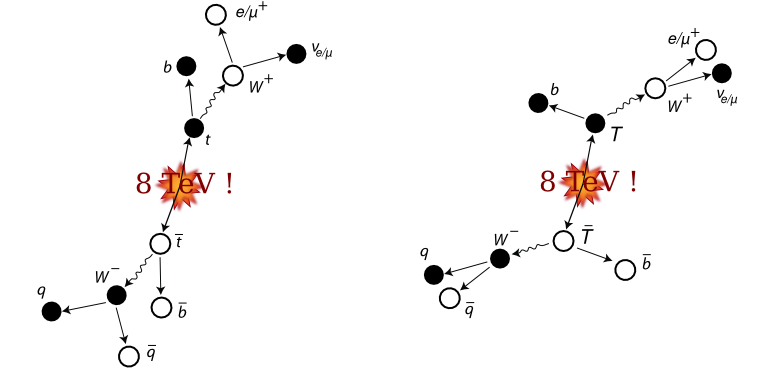
\includegraphics[width=0.85\textwidth]{wbx_analysis_14ifb/figures/kin}}
	\caption{Pictorial representation of the typical kinematic configuration
        for top pairs decays (left), where the boosted objects are the top
        quarks themselves, and vector-like top pairs decays (right), where the
        boosted objects are the $W$ bosons.\label{fig:boostedkin}}
\end{center}\end{figure}

In order to exploit this dynamic the angular separation of the final state
objects is considered. Since the $W$ boson decay
in the lepton channel cannot be completely resolved because of
the presence (or better, absence) of a neutrino, the analysis
focuses on the reconstruction of the $W$ boson that decays in the hadronic
channel, called \whad\ in the following.
The two jets from the decay of the \whad\ are expected to be
light flavored jets. At the preselection level at least
one \btag ged jet is required. Since two \btag ged jets are expected in
the final state and in order to avoid the loss in acceptance that would follow a strict
cut like requiring at least two \btag ged jets\footnote{Considering our choice
of the working point for the \btag ging \texttt{MV1} algorithm with a 70\%
efficiency, a selection requiring at least two \btag ged jets would result
in a 50\% selection efficiency.}, the two jets with the 
highest weight computed from the \btag ging algorithm are considered ``\bjet s''.
Amongst the light jets two cases are considered: either the two light flavoured
quarks were produced so close-by that after hadronization the jet reconstruction
algorithm identifies a single jet, or two jets are found close one to the other.
To account for the first category of events, jets with $\pt>250\gev$ and a mass
between 60~\gev\ and 120~\gev, an interval chosen to cover both the world-average 
$W$ and $Z$ boson masses values of $m_W = 80.4$~\gev\ and $m_Z = 91.2$~\gev\ and
hence increasing the acceptance for $T\to Zt$ events, are 
classified as \wi\ candidates. If no \wi\ candidates are found, jets are paired
in di-jet systems if their angular separation $\dr(j,j)$ is lower than 0.8 and, if
$p_T(jj)>200\gev$ and 
their invariant mass $m_{jj}$ lies in the same window as for the \wi\ candidates, they 
are taken as a \wii\ candidate.


\section{Event selection}\label{sec:wbxEVT}

Once $W$ bosons are reconstructed in the event like explained in 
Section~\ref{sec:boostedW}, if at least one candidate is found the 
event is kept and further selection cuts are applied.
If multiple candidates are found, the one with mass closest 
to the nominal $W$ boson mass is chosen as the hadronic $W$ boson
of the event. 
Since in the final selection the Standard Model background contributions
from $W$+jets, $Z$+jets, diboson, single-top and multi-jet events
are very small, it is chosen to show these backgrounds combined into a
single component called ``non-$t\bar{t}$''.
Figures~\ref{fig:mwhadI} and~\ref{fig:mwhadII} show the mass distribution
of the \wi\ and \wii\ candidates before the mass window cut is applied. The
number of \whad\ candidates after preselection is shown in
Figure~\ref{fig:nWhad}. 

For what concerns the $W$ boson decaying in the lepton channel, the \wlep\ candidate,
it is reconstructed using the lepton of the event and the $\met$, 
which is considered as the transverse momentum of the neutrino. 
In order to define the neutrino longitudinal momentum, it is required that
the invariant mass of the two-body system composed by the lepton and the neutrino 
equals the nominal $W$ boson. 
%up to a two-fold ambiguity. 
The neutrino 4-momentum is therefore set using the $\met$ $X$ and $Y$ components
while the $Z$ component $p_{Z_\nu}$ is computed from: 
\begin{eqnarray}
P_W^2 = (P_l + P_{\nu})^2 = M_W^2,
\end{eqnarray}
which after some work around gives:
\begin{eqnarray}
\alpha &=& \dfrac{1}{2}(M_W^2 - M_l^2) \\
\beta  &=& \alpha + p_{X_\nu}p_{X_l} + p_{Y_\nu}p_{Y_l} \\
\gamma &=& -\dfrac{\beta^2 - E_l^2 (p_{X_\nu}^2+p_{Y_\nu}^2)}{E_l^2-p_{Z_l}^2} \\
\lambda &=& 2\beta \dfrac{p_{Z_l}}{E_l^2-p_{Z_l}^2}\\
\delta  &=& \lambda^2 - 4\gamma
\end{eqnarray}
and finally results in two possible solutions for the 
$Z$ component of the neutrino momentum:
\begin{eqnarray}
p_{Z_\nu} = \frac{\lambda \pm \sqrt{\delta} }{2}.
\end{eqnarray}
The chosen solution is the one giving
%Trying to assign both $p_Z$ to the neutrino 4-momentum, we choose the solution for
the smallest difference between the reconstructed 
heavy quark mass for the
leptonic and hadronic side of the decays (see Section~\ref{sec:wbxDISCR} 
for the details on the invariant mass reconstruction).
In the case no real solution exists, the neutrino pseudorapidity 
is set equal to that of the lepton, since in the kinematic regime of interest  
the decay products of the $W$ boson tend to be collinear.

Once all the objects taking part to the event are identified,
the selections summarized in Table~\ref{tab:wbxselection} are
applied with the aim of rejecting as much Standard Model background
as possible. As can be seen in the table, two final selection called
\loose\ and \tight\ selections are proposed, the latter being a
subset of the former with two very restrictive cut applied on top of it.
The ``Signal Region'' (SR) label is applied to the selections
progressively reaching the \tight\ selection.

\begin{table}[tb]
\begin{center}
\begin{tabular}{lll}
\toprule
Selection & Signal Region & Requirements \\
\midrule
Preselection & & One electron or muon  \\
             & & $\met >20\gev$, $\met +m_{\rm T}>60\gev$ \\
             & & $\geq 4$ jets, $\geq 1$ $b$-tagged jets \\
\midrule
\loose\ selection & SR0 & Preselection  \\
                  & SR1 & +\hskip5ex$\geq 1~W_{\rm had}$ candidates \\
                  & SR2 & +\hskip5ex$\HT>800\gev$ \\
                  & SR3 & +\hskip5ex $\pt(b_1) > 160\gev$\\
                  & SR4 & +\hskip5ex$\pt(b_2) >80\gev$ \\
                  & SR5 ($\equiv$\loose) & +\hskip5ex$\Delta R(\ell,\nu)<1.2$ \\
\midrule
\tight\  selection & SR5 & \loose\ selection \\
     	      & SR6 &  +\hskip5ex min$\Delta R(\ell,b)>1.4$\\
              & SR7 ($\equiv$\tight) & +\hskip5ex min$\Delta R(W_{\rm had},b)>1.4$ \\
\bottomrule
\end{tabular}
\caption{Summary of event selection requirements.}
\label{tab:wbxselection}
\end{center}
\end{table}


After finding at least one \whad\ candidate (SR1), a variable called $\HT$ is defined
as the scalar sum of the lepton $\pt$, $\met$ and the $\pt$
of the four  highest-$\pt$ jets. This $\HT$ distribution peaks at 
$\sim 2 m_{\T}$ for signal events and is therefore pretty useful to
discriminate between the signal and the background, as clearly shown
in Figure~\ref{fig:HTAll}. A cut at $\HT>800\gev$ (SR2) is chosen as particularly
efficient in rejecting background while keeping signal events.
Considering then the boost inflicted to the bottom quarks from the heavy
vector-like top decay, cuts on the \btag ged jets are defined.
Figures~\ref{fig:pTb1} and~\ref{fig:pTb2} show the transverse momentum distributions
of the highest-$\pt$ $b$-jet candidate ($b_1$) and 
the next-to-highest-$\pt$ $b$-jet candidate ($b_2$).
The cuts chosen are $\pt(b_1) > 160\gev$ (SR3) and $\pt(b_2) >80\gev$ (SR4).
To further discriminate between signal and background,
the angular separation between the lepton and the reconstructed neutrino 
(shown in Figure~\ref{fig:DRlnu}) is
required to satisfy $\Delta R(\ell,\nu)<1.2$ (SR5). What was described up to now 
are the requirements that lead to Signal Region 5, i.e. the \loose\ selection, as was
also summarized in Table~\ref{tab:wbxselection}. In the \tight\ selection
two further cuts on the angular separation between the lepton and the \btag ged
jet giving the minimum value, $\min(\Delta R(\ell, b_{1,2}))$ (Figure~\ref{fig:DRlb}), 
and between the
\whad\ candidate and the \btag ged jet giving the minimum value, 
$\min(\Delta R(W_{\rm had}, b_{1,2}))$ (Figure~\ref{fig:DRWb}) are defined as
 $\min(\Delta R(\ell, b_{1,2}))>1.4$ (SR6) and 
$\min(\Delta R(W_{\rm had}, b_{1,2}))>1.4$ (SR7, i.e. \tight\ selection).
In Table~\ref{tab:cftab} the expected and observed yields in these SRs are
reported for the electron and muon channels combined. In Appendix~\ref{app:wbxSR}
the final discriminant variable (to be discussed in Section~\ref{sec:wbxDISCR})
is shown for data, background and signal in the selection steps through the
signal region.

\begin{table}[htb]\centering
        \begin{tabular}{l c c c c } \toprule
 & $T\bar{T}$ (600) chiral 		 & $t\bar{t}$ MC@NLO 		 & non-$t\bar{t}$ 		 & Data 		 \\ \midrule 
SR0  & $379.62 \pm 6.91$  & $201692.98 \pm 282.31$  & $59665.95 \pm 348.84$  & $261881.00 \pm 511.74$ \\ 
SR1  & $168.29 \pm 4.54$  & $6335.53 \pm 50.55$  & $1416.55 \pm 45.03$  & $8401.00 \pm 91.66$ \\ 
SR2  & $161.24 \pm 4.46$  & $1574.87 \pm 26.41$  & $563.56 \pm 29.77$  & $2359.00 \pm 48.57$ \\ 
SR3  & $138.34 \pm 4.13$  & $812.12 \pm 18.76$  & $296.14 \pm 20.11$  & $1223.00 \pm 34.97$ \\ 
SR4  & $106.45 \pm 3.63$  & $436.85 \pm 13.64$  & $121.19 \pm 13.66$  & $598.00 \pm 24.45$ \\ 
SR5  & $87.98 \pm 3.31$  & $263.72 \pm 10.38$  & $52.92 \pm 7.01$  & $348.00 \pm 18.66$ \\ 
SR6  & $67.11 \pm 2.90$  & $26.67 \pm 3.61$  & $21.97 \pm 3.69$  & $61.00 \pm 7.81$ \\ 
SR7  & $53.91 \pm 2.60$  & $10.03 \pm 2.49$  & $10.77 \pm 3.06$  & $37.00 \pm 6.08$ \\ 
\bottomrule\end{tabular}

        \caption{Selected number of events with their statistical error
        in the Signal Regions (see Table~\ref{tab:wbxselection} for the
        region definitions).}\label{tab:cftab}
\end{table}



Tables~\ref{tab:eff_loose} and~\ref{tab:eff_tight} 
summarize the acceptance times efficiency for the \loose\ and \tight\ selections, 
respectively,
separately for each of the allowed \TTbar decay modes that can enter
the selections and as a function of $m_{\T}$.
%background  is 21.7 events, while the expected signal from a chiral fourth-generation quark with $m_\T=600\gev$ is 53.9 events, resulting in a $S/\sqrt{B}=11.6$.

\begin{table}[htb]
\begin{center}
\begin{tabular}{l c c c c c c}
\toprule
 & \multicolumn{6}{c}{Decay mode} \\
$m_{\T}$ ($\gev$) & $WbWb$ & $WbZt$ & $ZtZt$ & $WbHt$ & $ZtHt$ & $HtHt$ \\
\midrule
350 & 0.48\% & 0.21\% & 0.11\% & 0.18\% & 0.06\% & 0.08\% \\
400 & 0.95\% & 0.34\% & 0.13\% & 0.26\% & 0.14\% & 0.08\% \\
450 & 1.79\% & 0.57\% & 0.24\% & 0.47\% & 0.22\% & 0.15\% \\
500 & 2.26\% & 0.89\% & 0.36\% & 0.68\% & 0.28\% & 0.21\% \\
550 & 3.25\% & 1.21\% & 0.52\% & 1.07\% & 0.46\% & 0.35\% \\
600 & 3.92\% & 1.64\% & 0.60\% & 1.34\% & 0.62\% & 0.58\% \\
650 & 4.20\% & 2.08\% & 1.08\% & 1.66\% & 0.82\% & 0.60\% \\
700 & 5.05\% & 2.42\% & 2.10\% & 2.01\% & 1.04\% & 0.76\% \\
750 & 5.17\% & 2.84\% & 1.46\% & 2.40\% & 1.27\% & 0.82\% \\
800 & 5.72\% & 3.35\% & 1.67\% & 2.69\% & 1.43\% & 1.18\% \\
\bottomrule
\end{tabular}
\caption{Acceptance times efficiency for different \TTbar decay modes as a function of $m_{\T}$ for the \loose\ selection.}
\label{tab:eff_loose}
\end{center}
\end{table}

\begin{table}
\begin{center}
\begin{tabular}{l c c c c c c}
\toprule
 & \multicolumn{6}{c}{Decay mode} \\
$m_{\T}$ ($\gev$) & $WbWb$ & $WbZt$ & $ZtZt$ & $WbHt$ & $ZtHt$ & $HtHt$ \\
\midrule
350 & 0.17\% & 0.023\% & 0.011\% & 0.022\% & 0.0018\% & 0.0072\% \\
400 & 0.46\% & 0.054\% & 0.011\% & 0.047\% & 0.023\% & 0.014\% \\
450 & 1.11\% & 0.14\% & 0.047\% & 0.11\% & 0.027\% & 0.054\% \\
500 & 1.38\% & 0.32\% & 0.068\% & 0.21\% & 0.065\% & 0.029\% \\
550 & 1.92\% & 0.45\% & 0.10\% & 0.34\% & 0.12\% & 0.11\% \\
600 & 2.45\% & 0.64\% & 0.10\% & 0.47\% & 0.18\% & 0.16\% \\
650 & 2.46\% & 0.74\% & 0.22\% & 0.60\% & 0.21\% & 0.19\% \\
700 & 3.21\% & 0.97\% & 0.24\% & 0.74\% & 0.27\% & 0.25\% \\
750 & 3.16\% & 1.06\% & 0.29\% & 0.94\% & 0.34\% & 0.29\% \\
800 & 3.57\% & 1.35\% & 0.30\% & 1.06\% & 0.38\% & 0.34\% \\
\bottomrule
\end{tabular}
\caption{Acceptance times efficiency for different \TTbar decay modes as a function of $m_{\T}$ for the \tight\ selection.}
\label{tab:eff_tight}
\end{center}
\end{table}





\begin{figure}[h!tb]\begin{center}
	\subfigure[]{\label{fig:mwhadI}
          	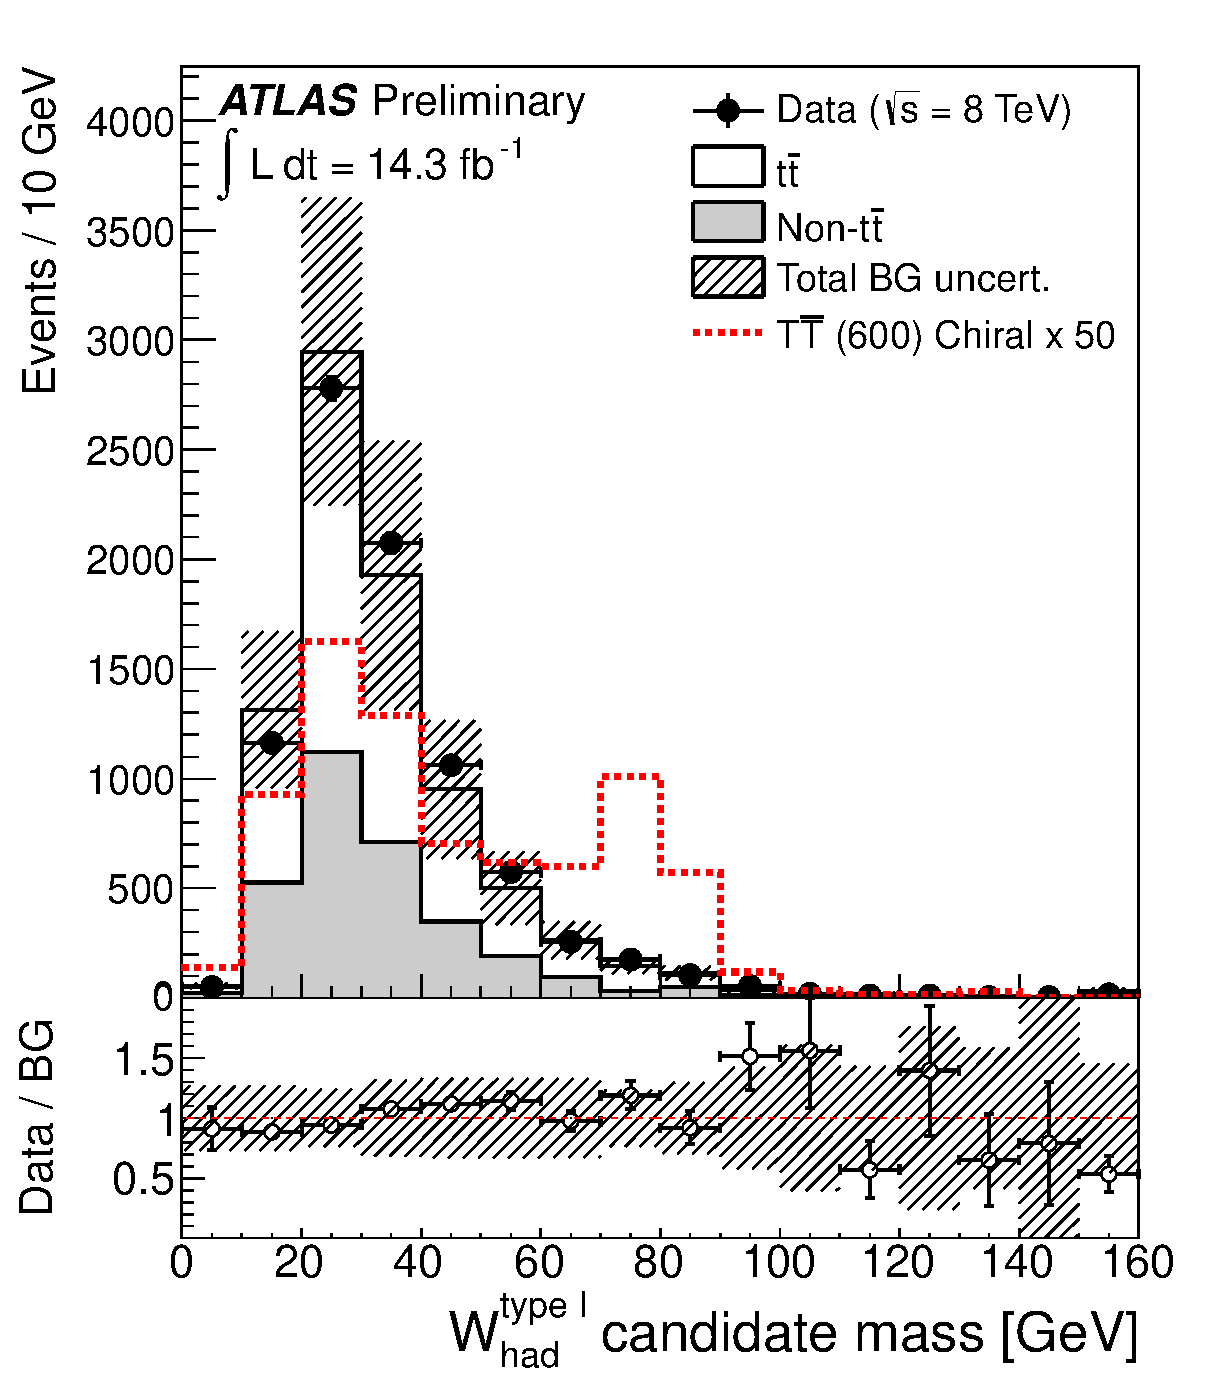
\includegraphics[width=0.47\textwidth]{wbx_analysis_14ifb/figures/confnoteplots/VLQAna_WbX_WpreselType1_M_ELEMUON_preselW_NOMINAL.eps}}
	\subfigure[]{\label{fig:mwhadII}
                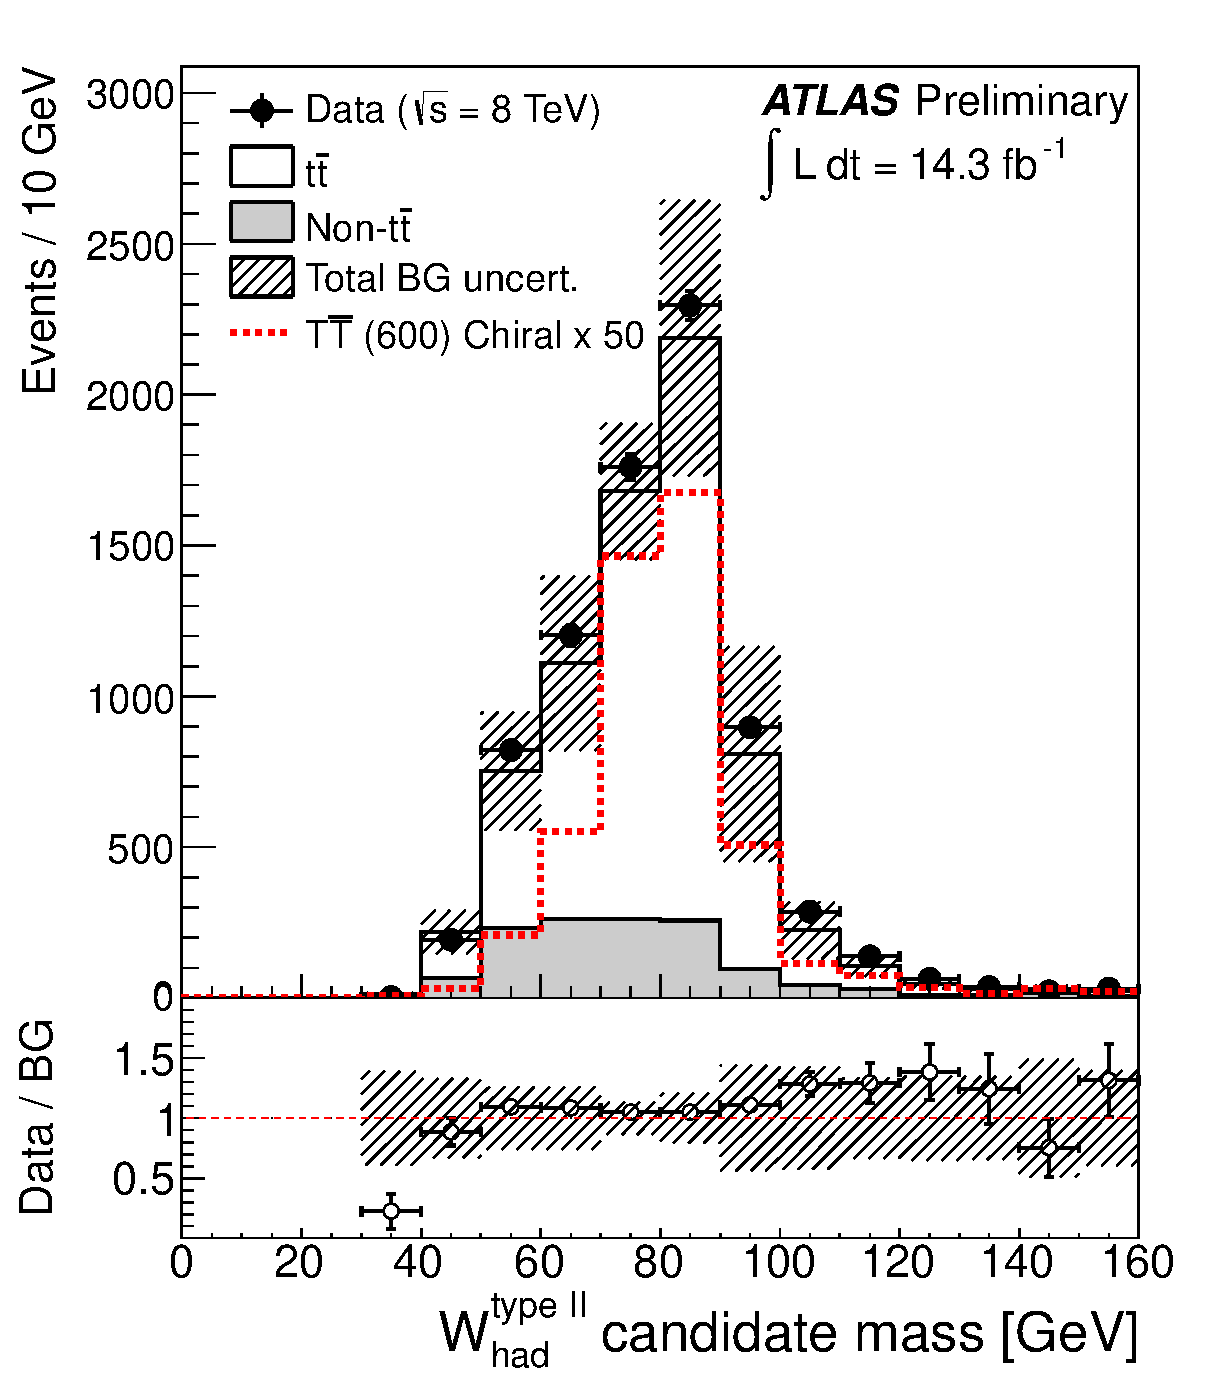
\includegraphics[width=0.47\textwidth]{wbx_analysis_14ifb/figures/confnoteplots/VLQAna_WbX_WpreselType2_M_ELEMUON_preselW_NOMINAL.eps}}
%	\caption[bla]{Distribution of the reconstructed mass for 
%        (a) \wi\ and (b) \wii\ candidates
%        for the combined $e$+jets and $\mu$+jets channels after preselection,
%        prior to apply the mass window cut.
%                The data (solid black points) are compared to the background 
        prediction from Standard Model (stacked histograms). 
        The total uncertainty on the background estimation (see 
        Section~\ref{sec:wbxSYS} for details) is shown as a black hashed band.
        The expected contribution from a chiral fourth-generation $T$ quark 
        with mass $m_{\T}=600\gev$, multiplied by a factor of 50, 
        is also shown (red dashed histogram).
        The lower panel shows the ratio of data to background prediction. 
        The overflow has been added to the last bin.

%        \label{fig:mwhad}}
%\end{center}\end{figure}
%\begin{figure}[h!bt]\begin{center}
	\subfigure[]{\label{fig:nWhad}
                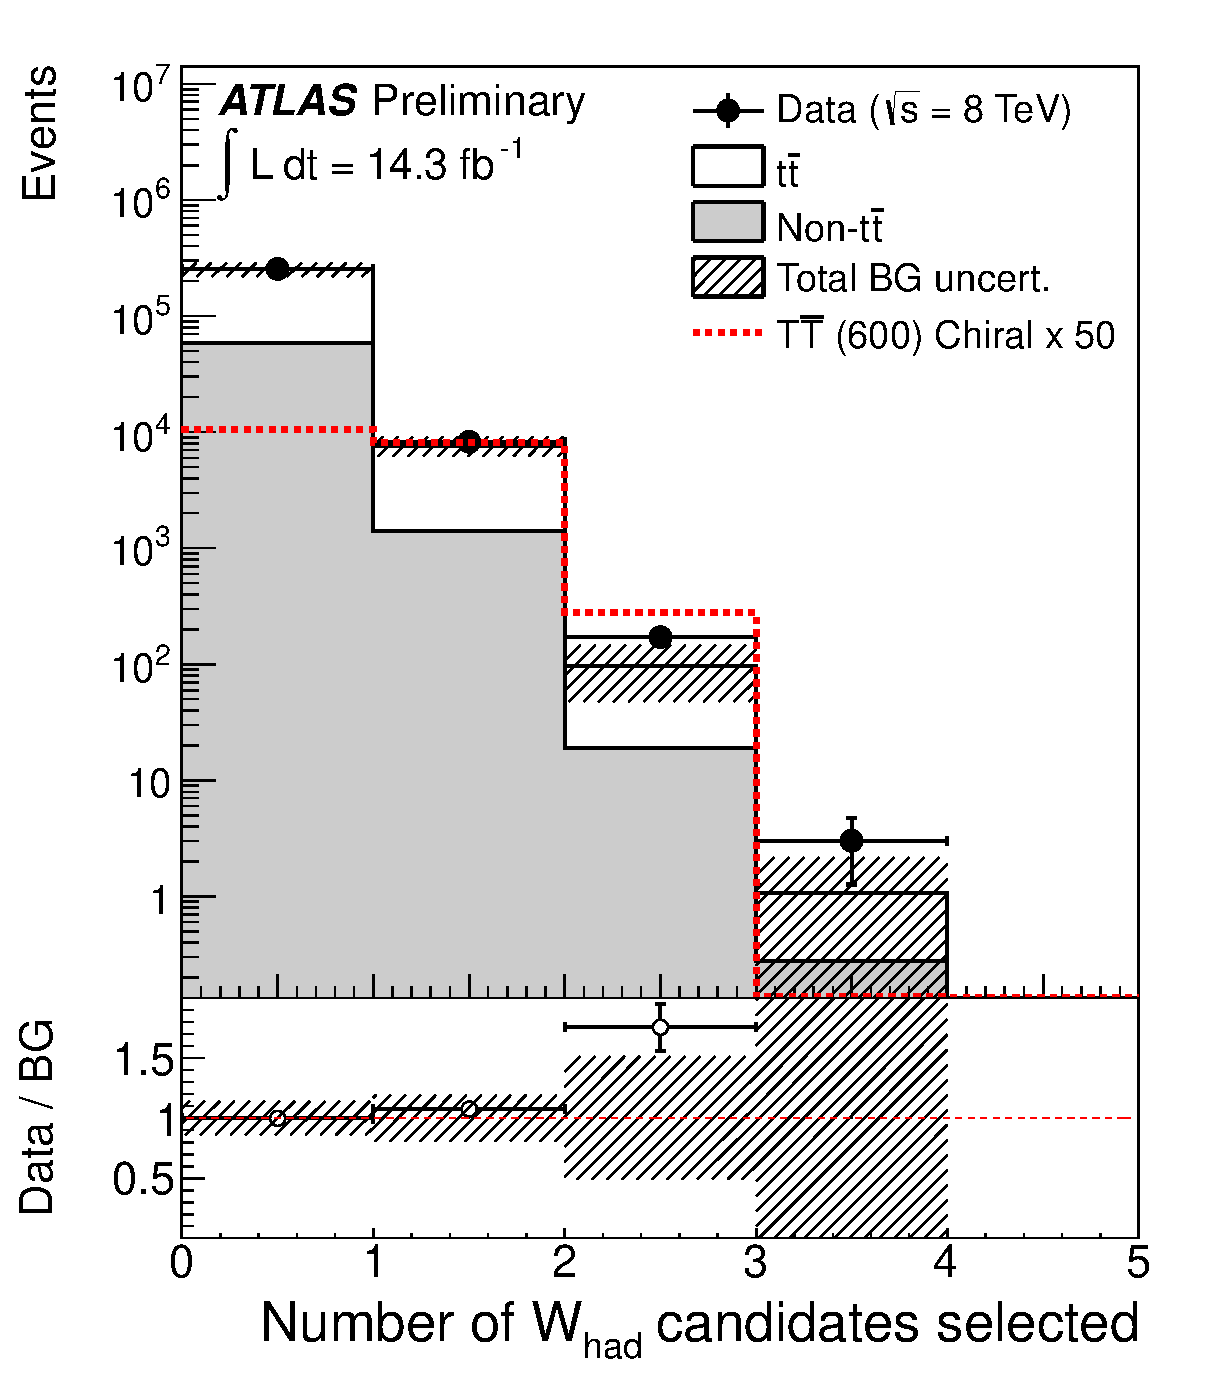
\includegraphics[width=0.45\textwidth]{wbx_analysis_14ifb/figures/confnoteplots/nWhad_ELEMUON_cutflow0_NOMINAL_logscale.eps}}
	\subfigure[]{\label{fig:HTAll}
                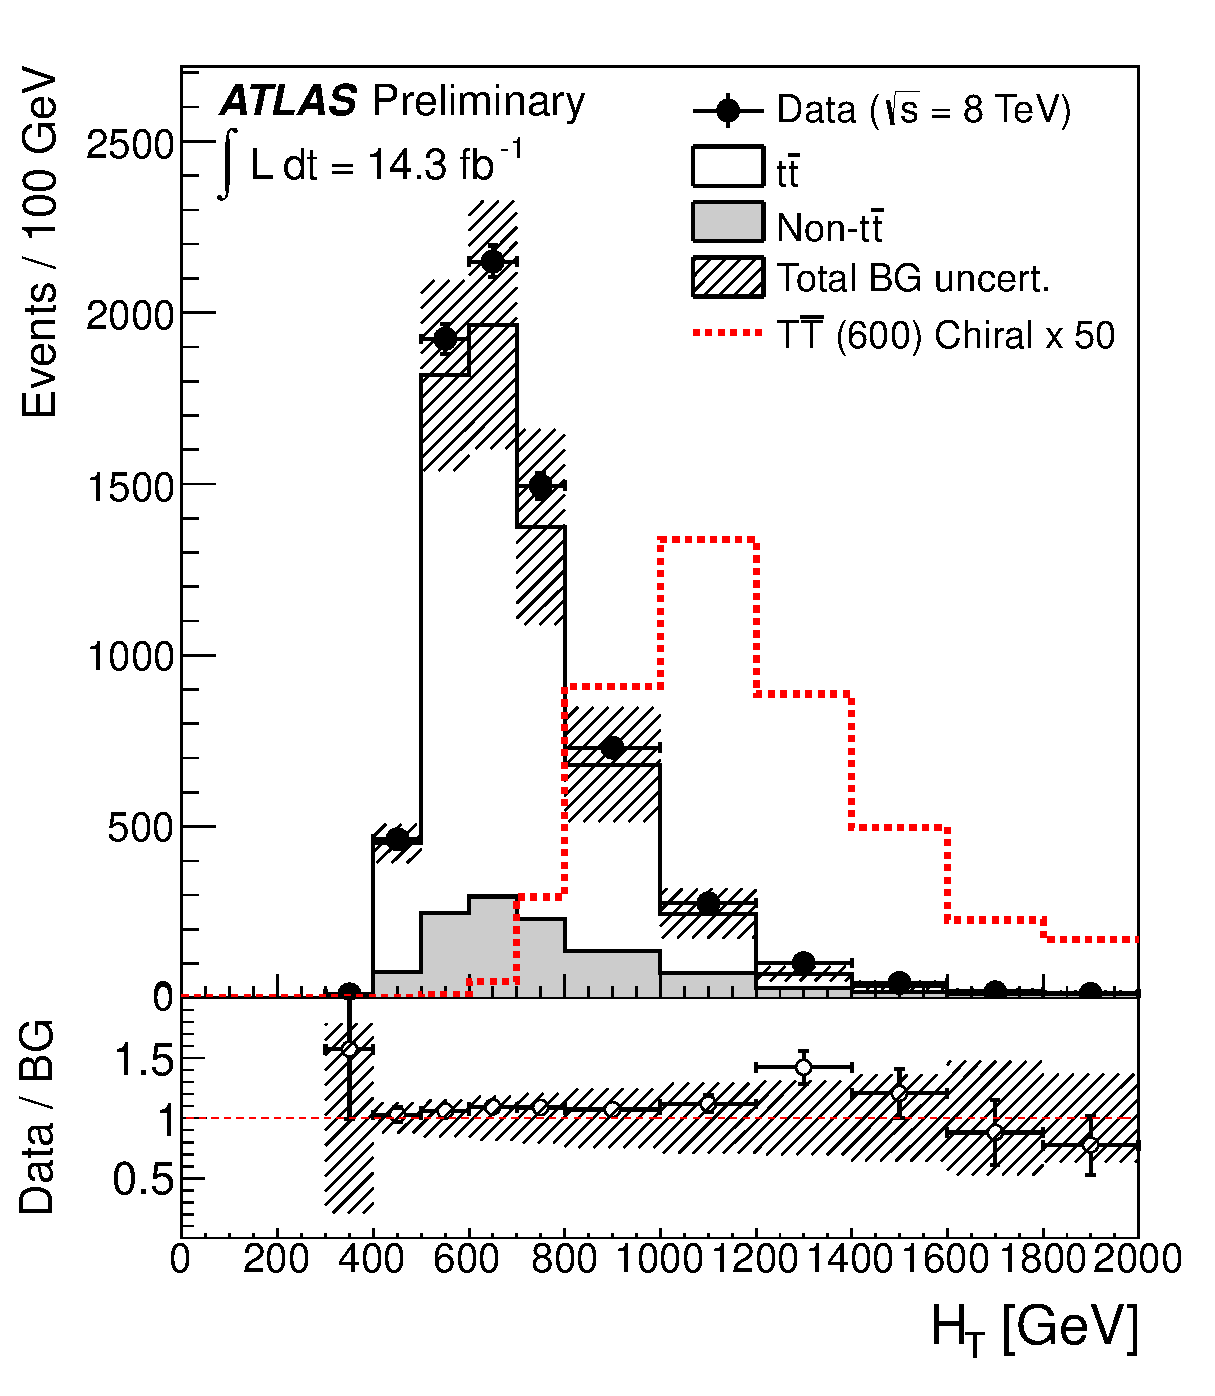
\includegraphics[width=0.45\textwidth]{wbx_analysis_14ifb/figures/confnoteplots/HTAll_ELEMUON_cutflow1_NOMINAL.eps}}
%        \caption[bla]{Distribution of (a) number of $W_{\rm had}$ candidates 
%        at the preselection level, and (b) $\HT$ after requirement of
        \caption[bla]{Distribution of the reconstructed mass for 
        (a) \wi\ and (b) \wii\ candidates
        for the combined $e$+jets and $\mu$+jets channels after preselection,
        prior to apply the mass window cut;
        distribution of (c) number of $W_{\rm had}$ candidates 
        at the preselection level, and (d) $\HT$ after requirement of
        $\geq 1$ $W_{\rm had}$ candidate, for the combined 
        $e$+jets and $\mu$+jets channels.
                The data (solid black points) are compared to the background 
        prediction from Standard Model (stacked histograms). 
        The total uncertainty on the background estimation (see 
        Section~\ref{sec:wbxSYS} for details) is shown as a black hashed band.
        The expected contribution from a chiral fourth-generation $T$ quark 
        with mass $m_{\T}=600\gev$, multiplied by a factor of 50, 
        is also shown (red dashed histogram).
        The lower panel shows the ratio of data to background prediction. 
        The overflow has been added to the last bin.

        \label{fig:mwhad_nWhad_HTAll}}
\end{center}\end{figure}

\begin{figure}[h!tb]\begin{center}
        \subfigure[]{\label{fig:pTb1}
                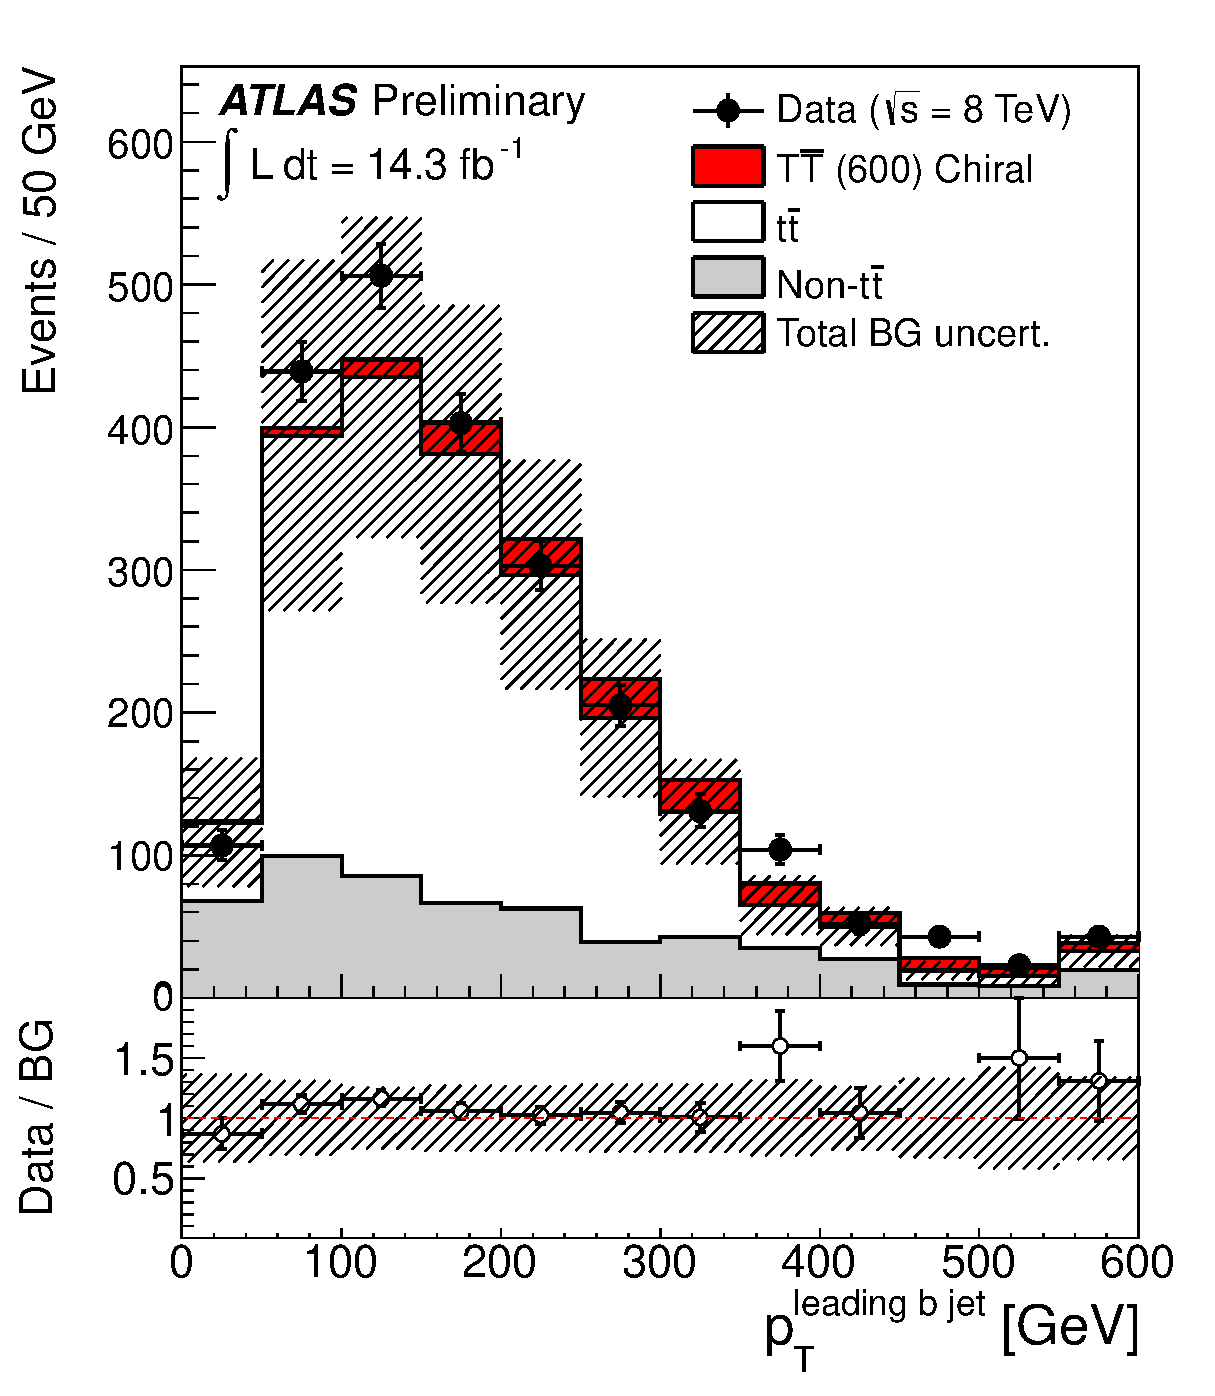
\includegraphics[width=0.45\textwidth]{wbx_analysis_14ifb/figures/confnoteplots/JetPtB1_ELEMUON_cutflow12_NOMINAL.eps}}
        \subfigure[]{\label{fig:pTb2}
                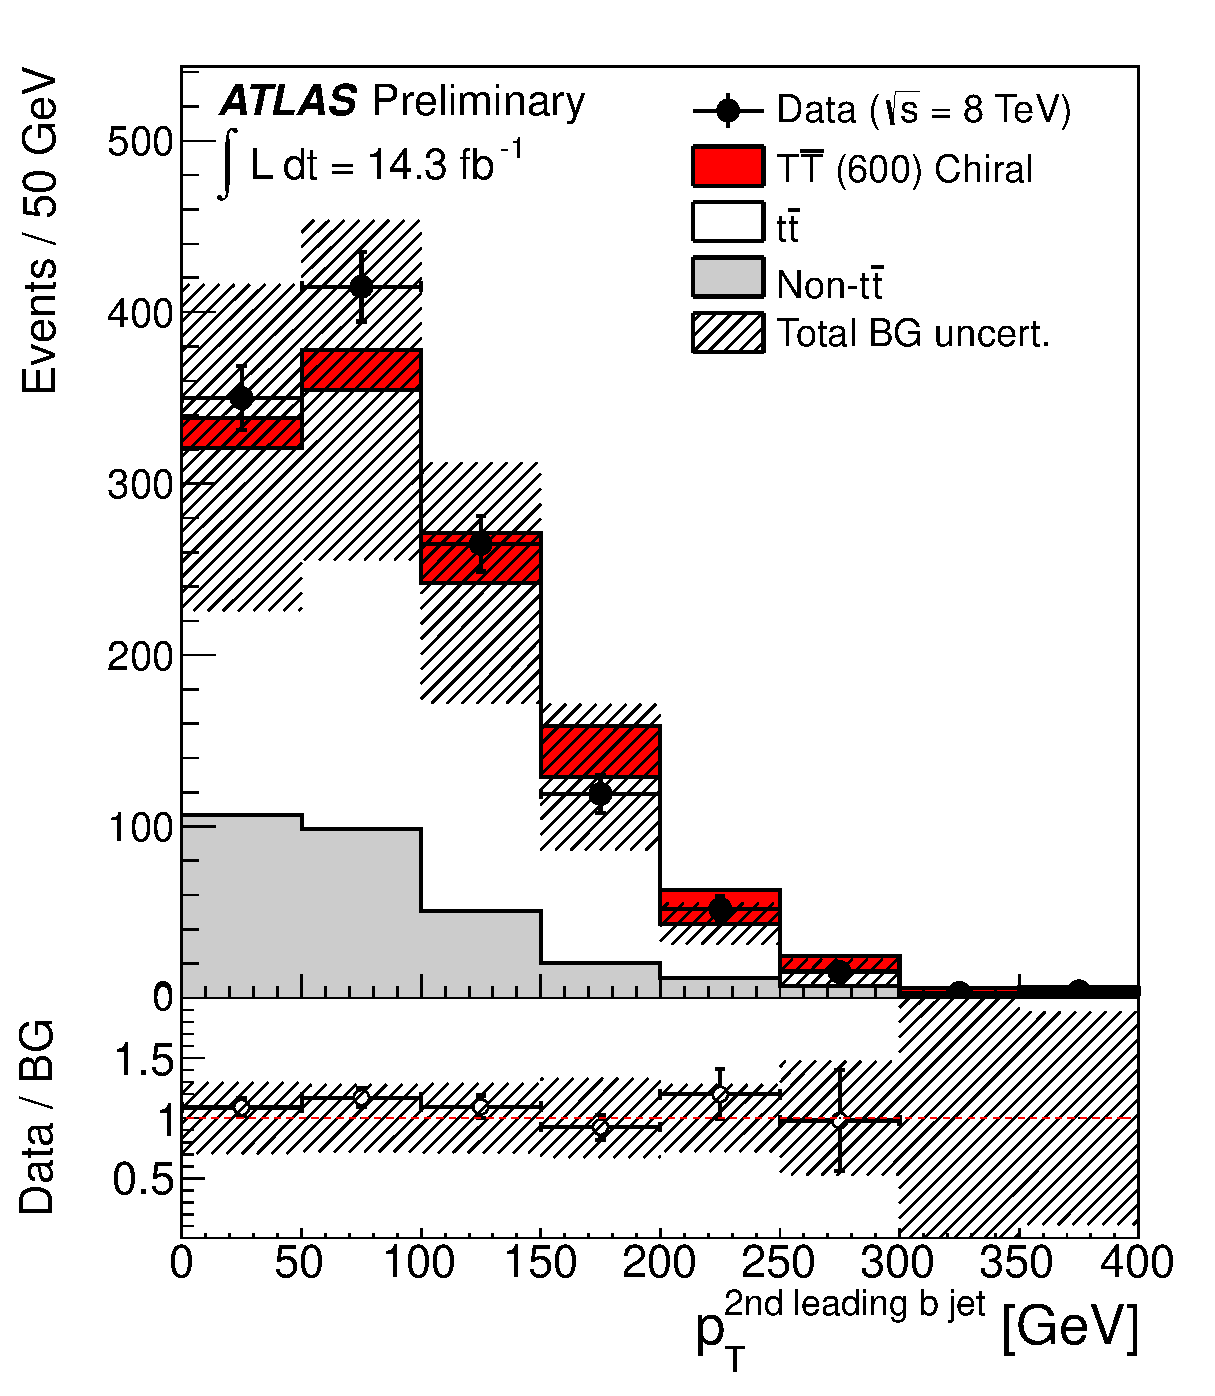
\includegraphics[width=0.45\textwidth]{wbx_analysis_14ifb/figures/confnoteplots/JetPtB2_ELEMUON_cutflow123_NOMINAL.eps}}
%        \caption[bla]{Distribution of (a) $\pt$ of leading $b$ jet candidate, $\pt(b_1)$, and (b) $\pt$ of subleading $b$ jet candidate, $\pt(b_2)$,
%for the combined $e$+jets and $\mu$+jets channels after all previous selection requirements (see text for details), 
%except for the requirements on $\pt(b_1)$ and $\pt(b_2)$ themselves.
%                The data (solid black points) are compared to the background 
        prediction from Standard Model (stacked histograms). 
        The total uncertainty on the background estimation (see 
        Section~\ref{sec:wbxSYS} for details) is shown as a black hashed band.
        The expected contribution from a chiral fourth-generation $T$ quark 
        with mass $m_{\T}=600\gev$, multiplied by a factor of 50, 
        is also shown (red dashed histogram).
        The lower panel shows the ratio of data to background prediction. 
        The overflow has been added to the last bin.

%\label{fig:pTb1_pTb2}}
%\end{center}\end{figure}
%\begin{figure}[h!tb]\begin{center}
	\subfigure[]{\label{fig:DRlnu}
                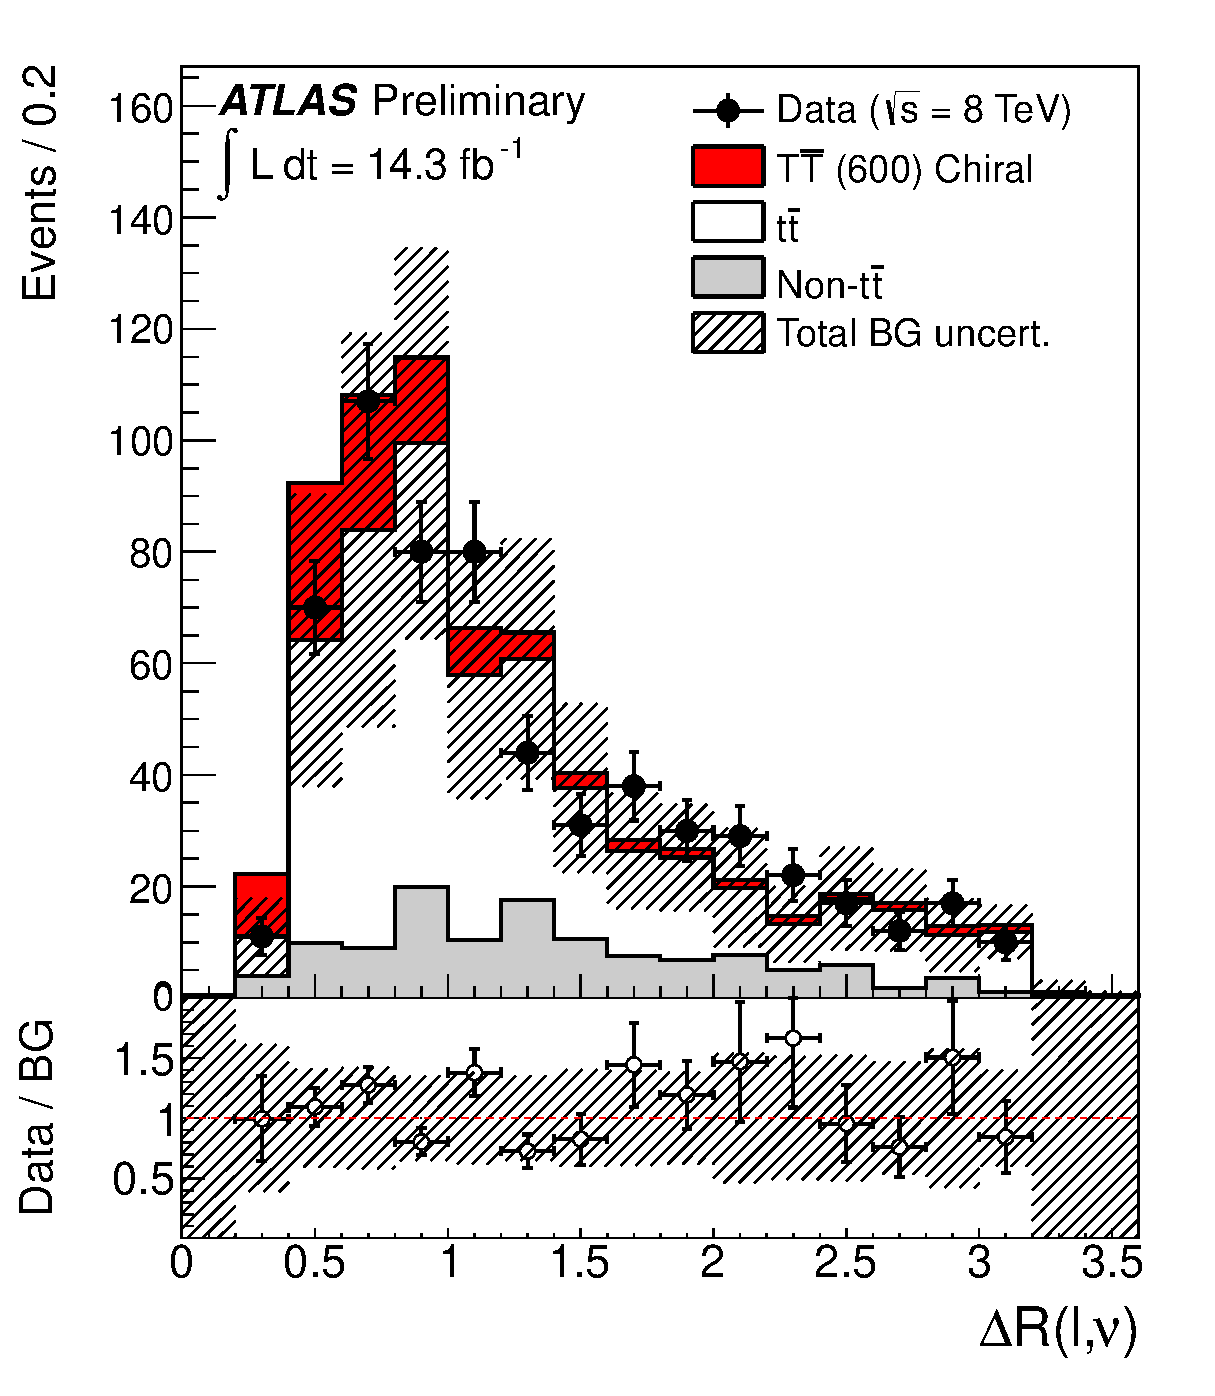
\includegraphics[width=0.45\textwidth]{wbx_analysis_14ifb/figures/confnoteplots/VLQAna_WbX_DRLepMet_ELEMUON_cutflow1234_NOMINAL.eps}}
	%\subfigure[]{\label{fig:DRlb}
        %        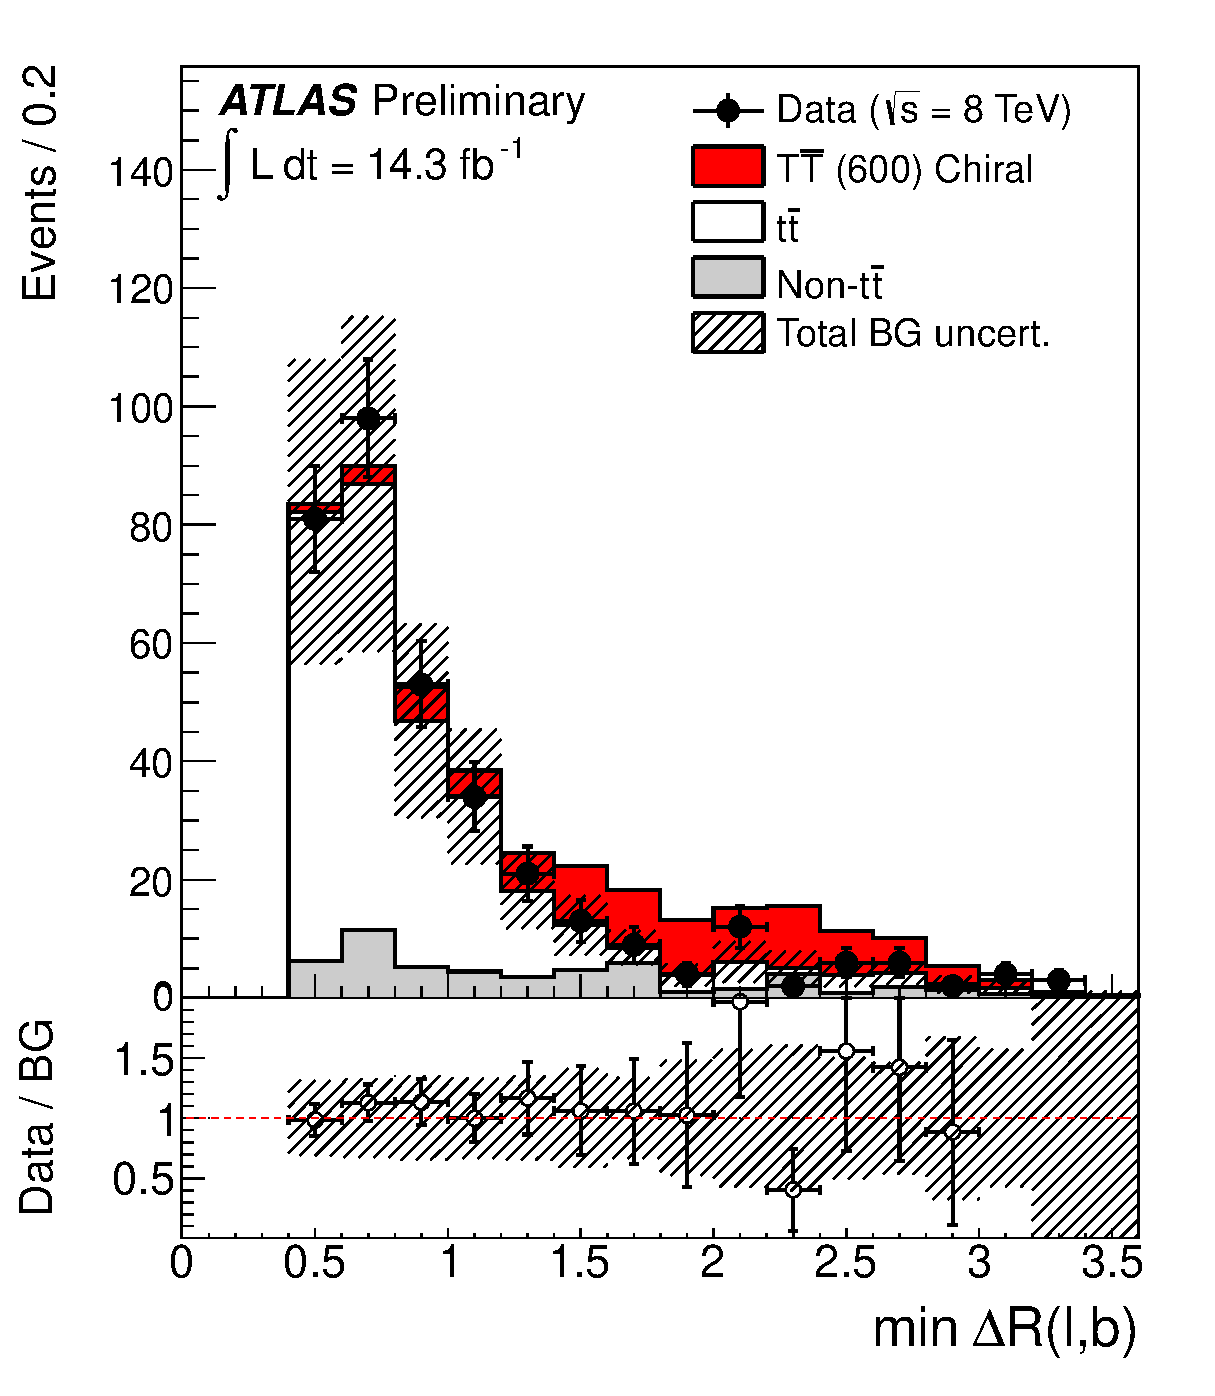
\includegraphics[width=0.45\textwidth]{wbx_analysis_14ifb/figures/confnoteplots/VLQAna_WbX_MinDRlb_ELEMUON_cutflow12345_NOMINAL.eps}}
        \caption[bla]{Distribution of (a) $\pt$ of leading $b$ jet candidate, $\pt(b_1)$, and (b) $\pt$ of subleading $b$ jet candidate, $\pt(b_2)$,
for the combined $e$+jets and $\mu$+jets channels after all previous selection requirements (see text for details), 
except for the requirements on $\pt(b_1)$ and $\pt(b_2)$ themselves;
%                \caption[bla]{Distribution of (a) $\Delta R(\ell,\nu)$ and (b) $\min(\Delta R(\ell, b_{1,2}))>1.4$ 
              distribution of (c) $\Delta R(\ell,\nu)$ and (d) $\min(\Delta R(\ell, b_{1,2}))>1.4$ 
for the combined $e$+jets and $\mu$+jets channels after all previous selection requirements (see text for details), 
except for the requirements on $\Delta R(\ell,\nu)$ and $\min(\Delta R(\ell, b_{1,2}))>1.4$  themselves.
                The data (solid black points) are compared to the background 
        prediction from Standard Model (stacked histograms). 
        The total uncertainty on the background estimation (see Section~\ref{sec:SystematicUncertainties} for details) is shown as a black hashed band.
        The expected contribution from a chiral fourth-generation 
        $\T$ quark with mass $m_{\T}=600\gev$ is also shown (red shaded histogram), 
        stacked on top of the Standard Model background. 
        The lower panel shows the ratio of data to Standard Model prediction. 
        The overflow has been added to the last bin.


\label{fig:pTb1_pTb2_DRlnu_DRlb}}
\end{center}\end{figure}


\begin{figure}[htb]\begin{center}
	\subfigure[]{\label{fig:DRlb}
                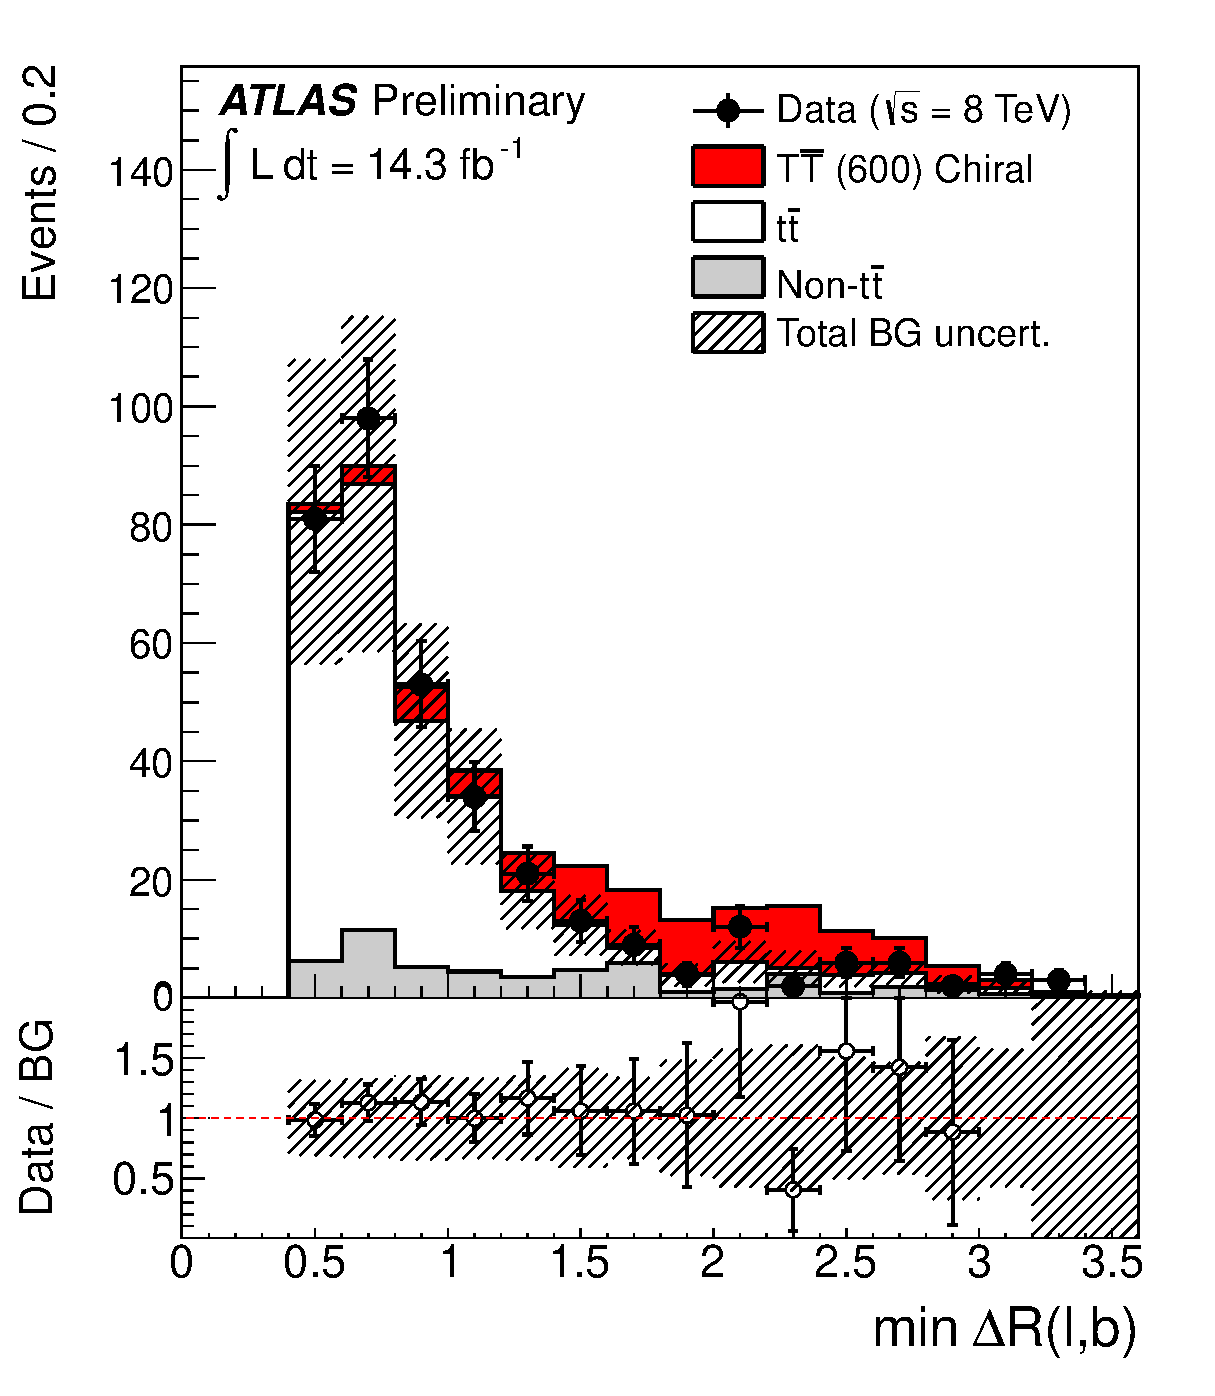
\includegraphics[width=0.45\textwidth]{wbx_analysis_14ifb/figures/confnoteplots/VLQAna_WbX_MinDRlb_ELEMUON_cutflow12345_NOMINAL.eps}}
	\subfigure[]{\label{fig:DRWb}
                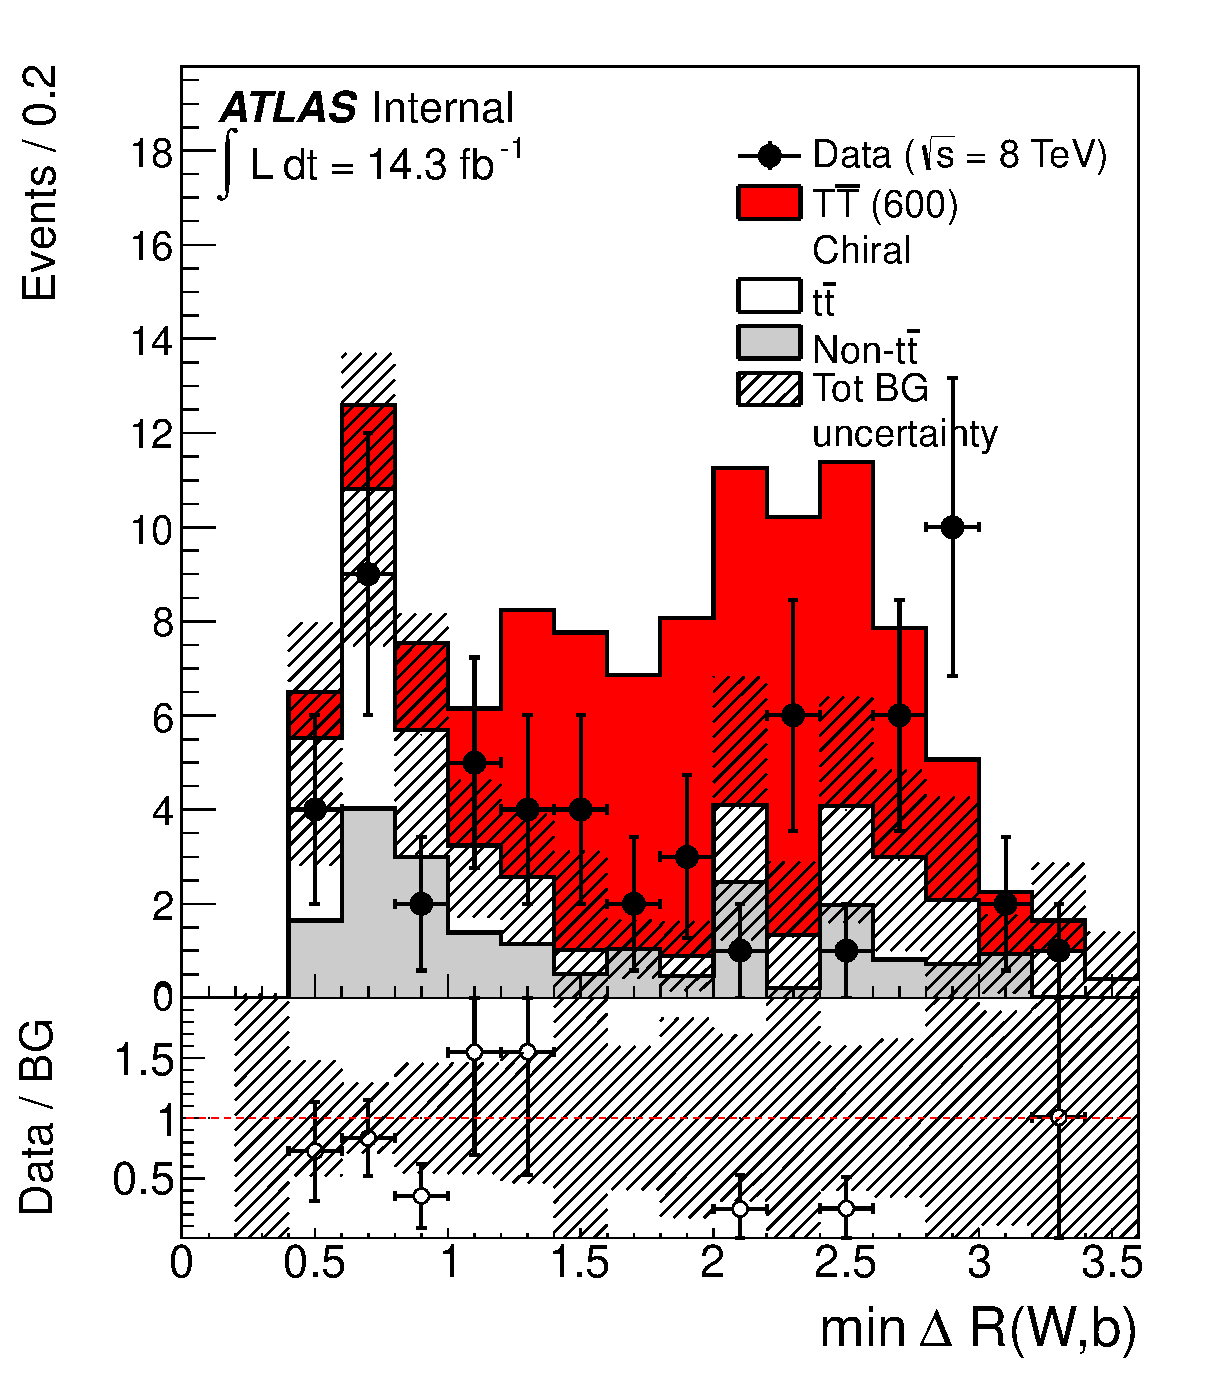
\includegraphics[width=0.45\textwidth]{wbx_analysis_14ifb/figures/confnoteplots/extra/VLQAna_WbX_MinDRWb_ELEMUON_cutflow123456_NOMINAL.eps}}
	\caption[bla]{Distribution of (a) $\min(\Delta R(\ell, b_{1,2}))$ 
        and (b) $\min(\Delta R(\whad, b_{1,2}))$
        for the combined $e$+jets and $\mu$+jets channels after all 
        previous selection requirements (see text for details), 
        except for the requirements $\min(\Delta R(\ell, b_{1,2}))>1.4$ and
        $\min(\Delta R(\whad, b_{1,2}))>1.4$ themselves, respectively.
        In the case of (a), this corresponds to the \loose\ selection.
                The data (solid black points) are compared to the background 
        prediction from Standard Model (stacked histograms). 
        The total uncertainty on the background estimation (see Section~\ref{sec:SystematicUncertainties} for details) is shown as a black hashed band.
        The expected contribution from a chiral fourth-generation 
        $\T$ quark with mass $m_{\T}=600\gev$ is also shown (red shaded histogram), 
        stacked on top of the Standard Model background. 
        The lower panel shows the ratio of data to Standard Model prediction. 
        The overflow has been added to the last bin.

}
\end{center}\end{figure}


In Table~\ref{tab:yields} the background estimates 
for the \loose\ and \tight\ selections are presented
together with the total predicted and observed yields
and the expectated number of events for two signal models, the
chiral and the singlet scenarios. 
The quoted uncertainties include both statistical and systematic contributions,
which are discussed in Section~\ref{sec:wbxSYS}.
The yields predicted from the Standard Model and the observed yields 
are in agreement within these uncertainties.
The absence of QCD multijet background from the table is due
to the fact that after the $\HT>800\gev$ requirement, the estimate
from the Matrix Method gives negative results, consistent with zero,
and is therefore set to zero.
It has been checked that its contribution is small ($\sim 0.2\%$ of the total)
even withouth the $\HT$ requirement, and is therefore considered negligible.

\begin{table}[h!tb]\centering
\begin{center}
  %\begin{tabular}{lrclrcl}
  \begin{tabular}{l  D{;}{\,\pm\,}{-1} D{;}{\,\pm\,}{-1} }
    \toprule
    & \multicolumn{1}{c}{\loose\ selection} 
    & \multicolumn{1}{c}{\tight\ selection}  \\\midrule
$t\bar{t}$    & 264;80 & 10;6 \\
$t\bar{t}V$   &  5.1;1.8 & 0.5;0.2 \\
$W$+jets   &  16;11 & 6;5\\
$Z$+jets   &  1.1;1.4 & 0.2;0.5 \\
Single top   &  30;7 & 4.4;1.6  \\
Dibosons &  0.21;0.15 & 0.06;0.05 \\
\midrule
Total background  & 317;90 & 21;9 \\
Data& 348 & 37  \\
%Data& \multicolumn{1}{c}{348\,\phantom{$\pm$}} & 37  \\
\midrule
$T\bar{T}(600\GeV)$ \\
Chiral fourth-generation &  88;10 & 54;7 \\
Vector-like singlet      & 41;4 & 20.3;2.2 \\
	\bottomrule\end{tabular}\caption{Number of observed events, integrated 
          over the whole mass spectrum, compared to the Standard Model expectation for
          the combined electron and muon channels after the \loose\ 
          and \tight\ selections.
          The expected signal yields  in two different scenarios, a chiral 
          fourth-generation $\T$ quark and a vector-like singlet $\T$ quark, 
          assuming $m_{\T}=600\gev$, are also shown.
          The quoted uncertainties include both statistical and 
          systematic contributions.}\label{tab:yields}
\end{center}
\end{table}



%\caption{\small{Number of observed events, integrated over the whole mass spectrum, compared to the SM expectation for
%the combined electron and muon channels after the {\sl loose} and {\sl tight} selections. 
%The expected signal yields  in two different scenarios, a chiral fourth-generation $\T$ quark and a vector-like singlet $\T$ quark, assuming $m_{\T}=600\gev$, are also shown.
%The quoted uncertainties include both statistical and systematic contributions.}}



%\input{figures/Cutflow/QCDtable/cutflowQCD.tex}



\section{Control regions}\label{sec:wbxCR}

In order to check the good modeling of Standard Model background
and its agreement with data in selection regions safely free from
possible signal presence, a number of ``signal-depleted'' regions (SDR) 
have been studied. These regions, summarized in Table~\ref{tab:SDRs},
progressively go from the preselection to the final selections keeping
away the signal by means of reverting one of the \tight\ selection cuts.
This allows to test regions enough close to the final signal selections
but still suppressing a potential signal contribution.
Plots of the comparisons between data and background for 
selected kinematic variables in each of these SDRs can be found in 
Appendix~\ref{app:wbxSDRs}.
In general, a reasonable agreement is found between data and Standard Model
prediction, with the $t\bar{t}$ contribution being modeled by the Monte Carlo 
generator \texttt{MC@NLO}, which was chosen after comparison with other
generators as providing the best description in the event configurations
this analysis is mostly interested in.
%A detailed comparison between data and three different full-simulation $t\bar{t}$ MC predictions: MC@NLO, POWHEG/PYTHIA and ALPGEN/HERWIG, can be found in Appendix~\ref{sec:DataMC_ttbarModeling} for  different signal-depleted regions. Overall MC@NLO provides the best description, which is the reason why it was adopted for default MC in this analysis. MC@NLO was also used in the previous result~\cite{atlas_WbWb_5fb_ljets}.

%%%%%%%%%%%%%%%
\begin{table}
\begin{center}
\begin{tabular}{ll}
\toprule
Region & Requirements \\
\midrule
SDR0 & preselection, $\geq 1$ $W_{\rm had}$ candidates, \\
            & reversed cut: $\HT<800\gev$ \\
SDR1 & preselection cuts, $\geq 1$ $W_{\rm had}$ candidates, \\
           &  reversed cut: $m_{\rm reco}<200\gev$ \\
SDR2 & \loose\ selection, \\
            & reversed cut: $\HT<800\gev$ \\
SDR3 & \loose\ selection, \\
            & reversed cut: $\pt < 160\gev$ and $\pt < 80\gev$ \\
SDR4 & \loose\ selection, \\
            & reversed cut: $\Delta R(\ell,\nu)>1.2$ \\
SDR5 & \loose\ selection, \\
            & reversed cut: $\min(\Delta R(W_{\rm had}, b_{1,2}))<1.4$ and $\min(\Delta R(\ell, b_{1,2}))<1.4$) \\
SDR6 & \loose\ selection, \\
            & reversed cut: $m_{\rm reco}<200\gev$ \\
SDR7 & \tight\ selection, \\
            & reversed cut: $\HT<800\gev$ \\
SDR8 & \tight\ selection, \\
            & reversed cut: $\pt < 160\gev$ and $\pt < 80\gev$ \\
SDR9 & \tight\ selection, \\
            & reversed cut: $\Delta R(\ell,\nu)>1.2$ \\
\bottomrule
\end{tabular}
\caption{List of signal-depleted regions considered.}
\label{tab:SDRs}
\end{center}
\end{table}
%%%%%%%%%%%%%%%


\section{Final discriminant: heavy quark reconstructed mass}\label{sec:wbxDISCR}

The discriminant variable chosen to build the binned log-likelihood ratio
for the statistical analysis of the search is the reconstructed mass of the
heavy vector-like top partner quark that decays into the boosted \whad, 
and is labelled as $m_{\rm reco}$. In order to build this variable the \whad\ 
candidate reconstructed as described in Section~\ref{sec:boostedW} has to
be paired with the associated bottom quark, to be chosen from the two
\btag ged jets selected in the analysis.
Another source of ambiguity comes from the computation of the longitudinal
momentum of the neutrino from the $W$ boson decay in the lepton channel.
The various combinations for the leptonic solution and the \btag ged jets
pairing are attempted and the one that in the end returns
the smallest difference between $m_{\rm reco}$ and $m(\wlep,b)$ is chosen
as final configuration.
In Figure~\ref{fig:mreco} the \mreco\ distribution in the \loose\
and \tight\ final selections is shown. From Figure~\ref{fig:mrecoLOOSE}
it is clear that this variable works well in discriminating between the
signal from the heavy quark and the backgrounds. Figure~\ref{fig:mrecoTIGHT}
instead shows a nice and clear peak from a chiral heavy top partner with mass
of 600~\gev\ with almost no background left after the \tight\ selection
requirements have been imposed.
As will be explained in Section~\ref{sec:wbxRES}, the \tight\ selection
shows the best sensitivity and therefore the distribution of 
Figure~\ref{fig:mrecoTIGHT} is the one chosen to derive the final test
statistics.

\begin{figure}[htb]\begin{center}
	\subfigure[]{\label{fig:mrecoLOOSE}
  	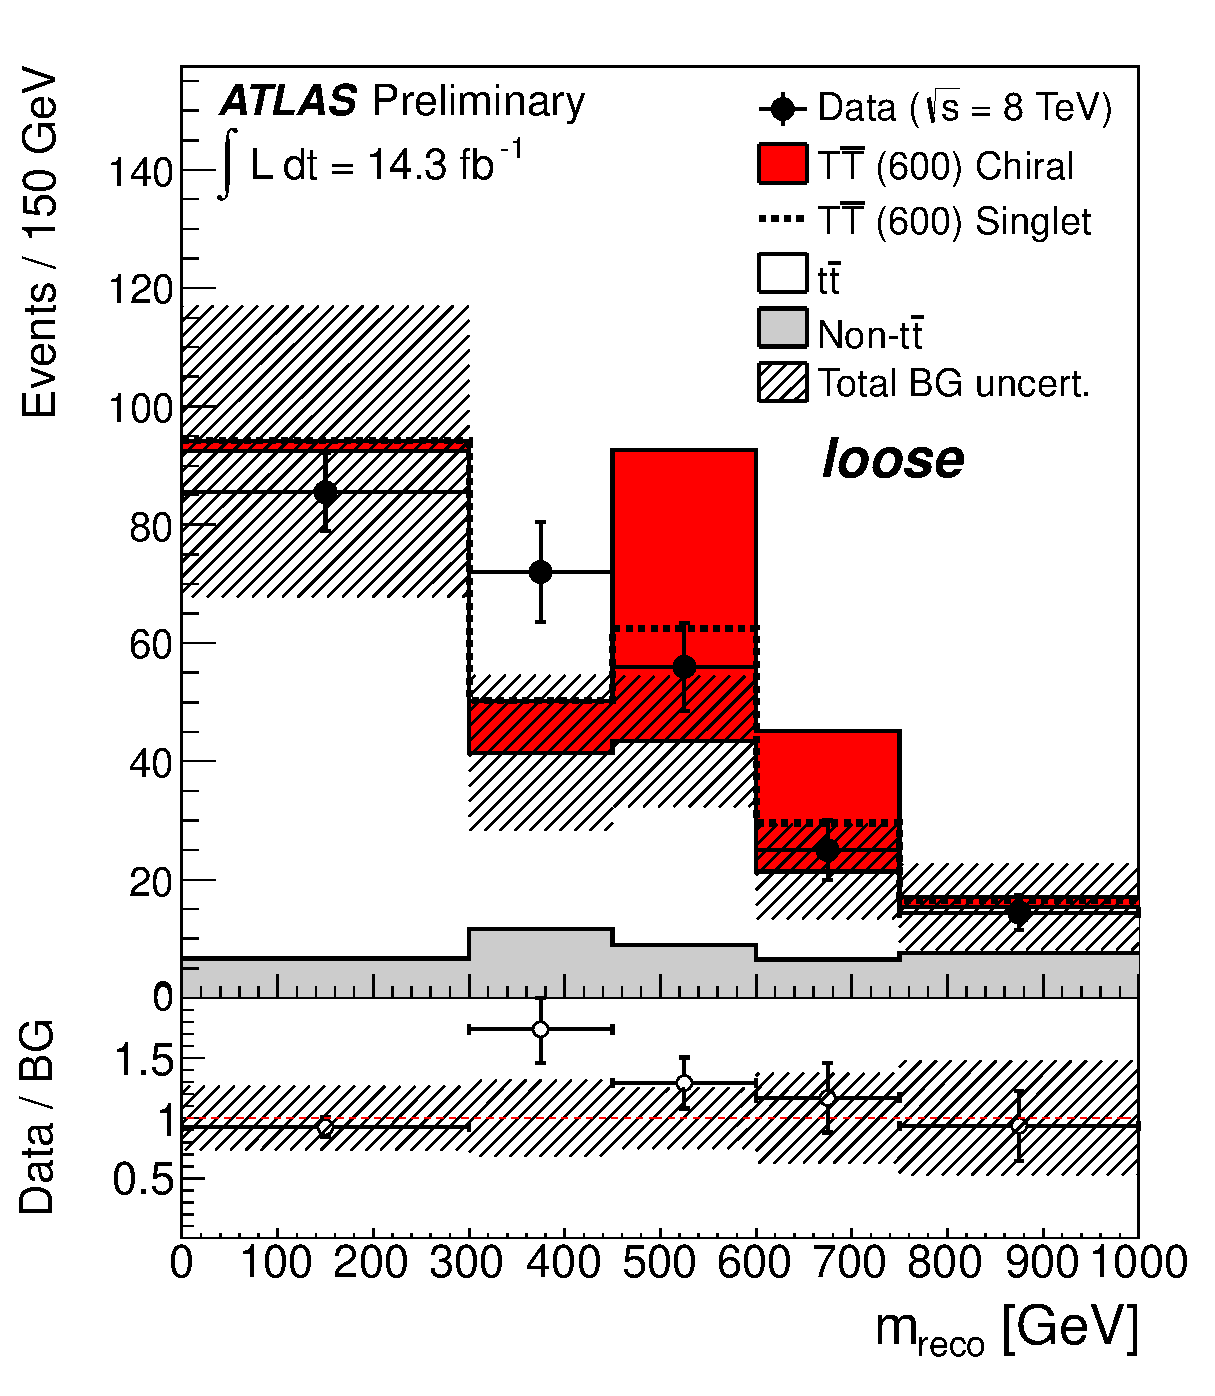
\includegraphics[width=0.45\textwidth]{wbx_analysis_14ifb/figures/confnoteplots/VLQAna_WbX_1W_MWb_4_ELEMUON_cutflow12345_NOMINAL.eps}}
	\subfigure[]{\label{fig:mrecoTIGHT}
  	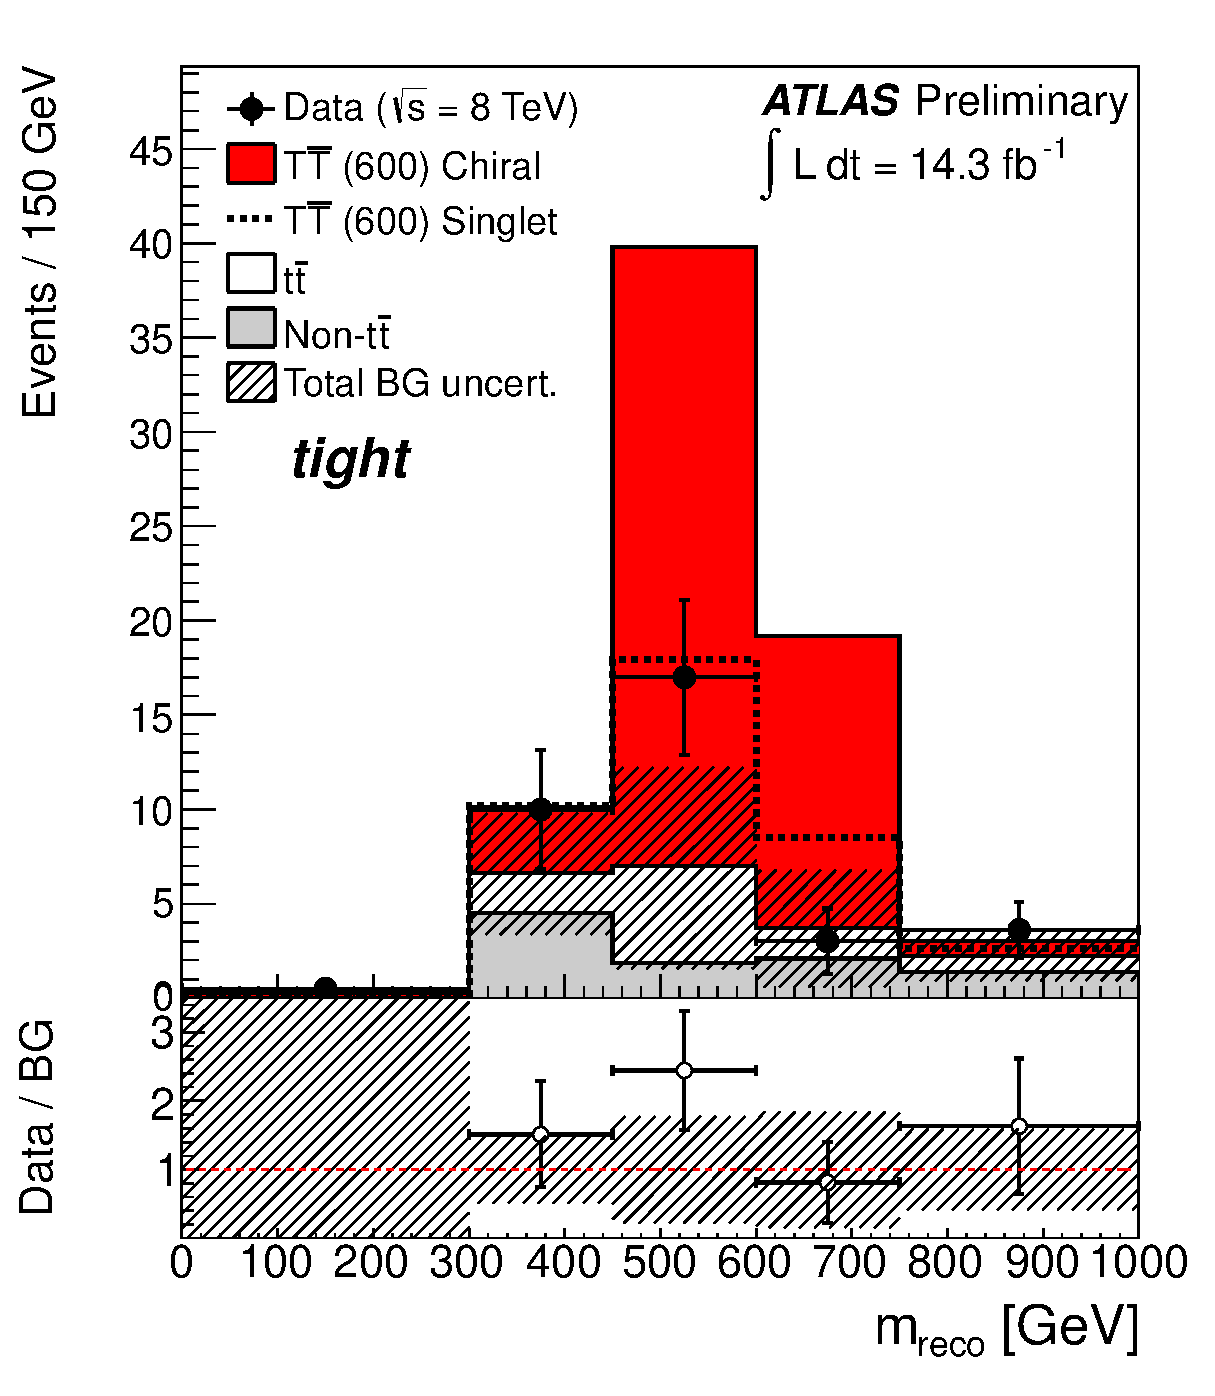
\includegraphics[width=0.45\textwidth]{wbx_analysis_14ifb/figures/confnoteplots/VLQAna_WbX_1W_MWb_4_ELEMUON_cutflow1234567_NOMINAL.eps}}
	\caption[bla]{Distribution of $m_{\rm reco}$  for the combined $e$+jets and $\mu$+jets channels after the (a) \loose\ and (b) \tight\ selection.
                The data (solid black points) are compared to the background 
        prediction from Standard Model (stacked histograms). 
        The total uncertainty on the background estimation (see Section~\ref{sec:SystematicUncertainties} for details) is shown as a black hashed band.
        The expected contribution from a chiral fourth-generation 
        $\T$ quark with mass $m_{\T}=600\gev$ is also shown (red shaded histogram), 
        stacked on top of the Standard Model background. 
        The lower panel shows the ratio of data to Standard Model prediction. 
        The overflow has been added to the last bin.

\label{fig:mreco}}
        %The shaded area represents the total background uncertainty (see Section~\ref{sec:SystematicUncertainties} for details). Also shown, stacked on top of the Standard Model background, is the expected contribution from signal corresponding to a chiral $\T$ quark with mass $m_{\T}=600\gev$.}
\end{center}\end{figure}


%\section{}\label{sec:}

\section{Systematics}\label{sec:wbxSYS}

%\subsection{Technical Details}
The general aspects of the systematic uncertainties considered
in the \wbx\ and \htx\ analyses were illustrated
in Section~\ref{sec:systematics}, here the traits specific to the
\wbx\ analysis will be described.

\subsection{Merging of non-$t\bar{t}$ Backgrounds}

The very stringent cuts defined to select signal and reject
background work so well that very low statistics is left for
``non-$t\bar{t}$'' backgrounds ($W+$jets, $Z+$jets, dibosons, single top, 
$t\bar{t}V$)\footnote{The prediction for QCD multi-jet background contribution
is negative and consistent with zero and is then set to zero.}.
This can lead to problems with the treatment of some systematic uncertainties as
e.g. an empty bin in the nominal case might have non-zero content in the
systematically varied sample. For this reason, considering that no resonances
are expected for these backgrounds, these \nontt\ samples are merged into
a single component. Systematic uncertainties like cross-section normalization,
which are specific for each background, are applied to the single component
and the nominal version of the other samples are added to obtain
a varied histogram.
For the \nontt\ background all systematic uncertainties are
treated as normalization-only.

%Contrary to what was described in Table~\ref{tab:sys}, all systematics are considered as normalization only for this small-background component. For the {\sc Tight} selection, we take the values derived from the {\sc Loose} selection, as we do not expect significant difference between the two cases.

\subsection{???Statistical uncertainty of the MC samples???}

The statistical uncertainty of the MC samples is taken into account when computing our likelihoods.
The {\sc mclimit} flag used is 2, meaning we consider the uncertainties as given by the uncertainties of the templates. 
This allows us to correctly estimate the statistical uncertainty when many templates are merged together with different weights, such as in
the case of the merged non-$t\bar{t}$ background.

\subsection{Profiling of Systematic Uncertainties}

In general no profiling of systematic uncertainties is performed, with
the only exception of the overall \ttbar\ yield in the analysis in the
\loose\ channel, where the low \mreco\ sideband dominated by the
\ttbar\ background contribution (see 
Figure~\ref{fig:mrecoLOOSE}) helps constraining the fluctuations.

\subsection{Jet energy scale}\label{sec:wbx_syst_jes}
Concerning the analysis performed in the \tight\ channel,
we recall here (see Section~\ref{sec:syst_jes} for details)
that it was chosen to treat the systematic uncertainties from
jet energy scale as a single component. Even with this treatment
large unphysical bin-to-bin fluctuations are observed
in the $m_{\rm reco}$ distribution for both $t\bar{t}$ and non-$t\bar{t}$
backgrounds in the \tight\ selection when the varied distributions
are compared with the nominal one. In order to overcome this issue
and the related noise that it would inject in the analysis, two different
approaches are followed for the $t\bar{t}$ and the non-$t\bar{t}$ background:
for the former, the systematic uncertainty shape is taken from the smoother
(because of the higher statistical population) template of the \loose\
channel, while in the case of the latter, where no resonances are expected,
a flat distribution is assumed and the systematic variation is taken as
normalization-only.
%Appendix~\ref{app:JEScomp} documents a study on the impact of each of the JES nuisance parameters on the normalisation and shape of the 
%reconstructed Higgs boson mass and $H_{Thad}$ distributions for $t\bar{t}H$ signal and $t\bar{t}$+jets background background in different
%jet multiplicity bins used in the analysis.
%Such study has resulted in a simplified prescription for the JES uncertainty breakdown for this analysis than involves a total
%of 9 nuisance parameters. 

\subsection{Jet energy resolution}
In addition to the general treatment explained in Section~\ref{sec:syst_jer},
%%%JER
for the $t\bar{t}$ and non-$t\bar{t}$ backgrounds 
the same behaviour is observed in the \tight\ channel
as for the systematic variations from the jet energy scale uncertainties.
Therefore the same treatment as previously outlined in 
Section~\ref{sec:wbx_syst_jes} is applied in order to 
reduce the impact on the analysis from
large unphysical statistical fluctuations.

\subsection{Jet Mass Scale and Resolution??? don't we compute it from the 4-vec???}
The jet mass is used  to identify the most energetic hadronically-decaying $W$ bosons that have been reconstructed as  single jets
($W_{\rm had}^{\rm type\;I}$ candidates). The uncertainties affecting the jet mass had been studied in the previous analysis at $\sqrt{s}=7\tev$ 
(see Section  8.2.7 in Ref.~\cite{atlas_WbWb_5fb_ljets_backup}. At the time, the existing jet mass scale/resolution uncertainties had been derived for larger anti-$k_t$ jets 
($R=1.0$) and in release 16~\cite{jet_mass_2011} and were believed to be conservative when applied to smaller $R=0.4$ jets using the 
refined calibration from release 17.  The jet mass scale uncertainties used in Ref.~\cite{atlas_WbWb_5fb_ljets_backup} were
4.5\% for jets with $\pt<400\gev$ and 6\% for $\pt>400\gev$ (from Table 18 in Ref.~\cite{jet_mass_2011}). The jet mass resolution
uncertainty used was 20\%, independent of jet $\pt$ (from Table 18 in Ref.~\cite{jet_mass_2011}). 
The propagation of these uncertainties in the previous analysis led to a degradation in the expected sensitivity of only a few $\gev$
(compare yellow and light blue curves in Fig. 25(b) of Ref.~\cite{atlas_WbWb_5fb_ljets_backup}). Given the small impact on the
sensitivity of an almost identical analysis at $\sqrt{s}=7\tev$ of what was judged to be a conservative uncertainty at the time, and since
no recommendation for  $R=0.4$ jets currently exists,  this uncertainty is currently being neglected.

\subsection{\Wboson/\Zboson+jets Normalisation}
\label{sec:syst_vjetsnormWBX}
The $W$/$Z$+jets cross sections as computed at the
leading-order in the
\texttt{Alpgen} generator framework
are affected by large uncertainties.
It was explained in Section~\ref{sec:Wjetsnorm}
that the overall $W$+jets normalization is 
corrected using data-driven methods 
performing the estimation in each jet multiplicity
bin (in the case of the \wbx\ analysis, the 4 jet bin
and the $\geq 5$ jet bin) in order to get the best
possible evaluation for the $W$+jets background contribution.
Additional uncertainties come from the fractions of $Wb\bar{b}$, $Wc\bar{c}$ and $Wc$
events and from their extrapolation from 2-jet events to higher jet multiplicity. 
The total uncertainty on the estimated $W$+jets normalization
in the \tight\ channel, as obtained from the  sum in quadrature 
of the above contributions, is of $\sim$30\%.



\subsection{$t\bar{t}$ Modelling}
\label{sec:systematic_ttbarmodel}

In order to evaluate the effect of systematic uncertainties 
affecting the modelling of the $t\bar{t}$ background from the
\texttt{MC@NLO} generator, the following factors are considered
in the \wbx\ analysis: the choice of NLO event generator;
the modeling of initial and final state radiation from QCD
precesses; the choice of parton shower and fragmentation models.

Concerning the NLO event generator choice, the effect of 
systematics uncertainties on the parton-level modeling of the
$t\bar{t}$ events is evaluated by comparing the distributions from two 
NLO Monte Carlo generators, namely \texttt{MC@NLO} (used for the nominal 
prediction in the \wbx\ 
analysis) and \texttt{PowHeg}, both interfaced to \texttt{Herwig} for
parton showering.  This choice is based on detailed comparisons
between data and Monte Carlo Standard Model backgrounds in a number 
of control regions, often defined starting from the \loose\ selection 
but with one of the cuts inverted to reject a possible signal contribution. 
In these studies three different $t\bar{t}$ generators, \texttt{MC@NLO}, \texttt{PowHeg} and
\texttt{Alpgen} were compared. In general, it was found that 
data was bracketed by \texttt{MC@NLO} and \texttt{PowHeg} predictions,
with \texttt{MC@NLO} providing the best description overall, which 
motivated its choice as the main $t\bar{t}$ generator for this analysis. 
In contrast, \texttt{Alpgen} was found to be the most inconsistent 
model with data, predicting yields above \texttt{PowHeg}, which 
motivated its rejection
as a valid alternate $t\bar{t}$  model in the kinematic region 
explored by this analysis.

Differences between \texttt{MC@NLO} and \texttt{PowHeg} arise from 
the details on how the NLO calculation is interfaced with the parton 
shower, resulting in \texttt{PowHeg} predicting higher
jet multiplicities than \texttt{MC@NLO}. The two samples used for the
comparison have been processed through a fast simulation of the detector,
and the difference in shape and normalization from these two samples of
\texttt{PowHeg}+\texttt{Herwig} 
and \texttt{MC@NLO} is symmetrised and propagated to the 
\texttt{MC@NLO} fully simulated sample as systematic uncertainty. 
The resulting uncertainty on the $t\bar{t}$ yield in the \tight\ selection 
is 48\%, and is the higher contribution to the total uncertainty
on the $t\bar{t}$ background. The same uncertainty in the \loose\ selection 
is 16\%. The significant
increase in the uncertainty for the \tight\ selection 
is mainly due to the increase in jet multiplicity in the
sample simulated with \texttt{PowHeg} with respect to the
one simulated with \texttt{MC@NLO}, 
which leads to a larger rate of misreconstructed $W_{\rm had}$ 
candidates. This makes the final cut of 
$\min(\Delta R(W_{\rm had}, b_{1,2}))>1.4$ cut less 
effective in discriminating signal and background than in the 
case of the nominal \texttt{MC@NLO}.

To assess the systematic uncertainty on the modeling of 
initial state (ISR) and final state radiation (FSR), dedicated
$t\bar{t}$ samples are generated with \texttt{AcerMC}
combined with \texttt{Pythia}, using modified \texttt{Pythia} parameters 
%%%yes?no?
(PARP(67), PARP(64) and PARP(72)) 
in order to increase or reduce the amount of parton shower. 
The range of variation for these parameters is chosen to be 
consistent with existing measurements such as the gap fraction in dileptonic 
$t\bar{t}$ events~\cite{ttjet} and jet shapes in QCD multijet events~\cite{morelessPS}.  
These samples have been processed through a fast simulation
of the detector. Half the difference between these alternate samples is symmetrized 
and propagated to the \texttt{MC@NLO} fully-simulated sample, resulting in a
systematic uncertainty on the $t\bar{t}$ yield in the \tight\ channel of 8.8\%.

\paragraph{Parton-Shower and Fragmentation Models:}
Finally, systematic uncertainties on the simulation 
of the parton shower and fragmentation models chosen 
are studied by comparison of two different hadronisation 
models applied to the same parton level generator: 
\texttt{PowHeg}+\texttt{Herwig} vs \texttt{PowHeg}+\texttt{Pythia}, 
both samples being processed through a fast simulation of the detector.
The relative difference measured between 
\texttt{PowHeg}+\texttt{Herwig} and \texttt{PowHeg}+\texttt{Pythia} is 
then symmetrised and propagated to the 
\texttt{MC@NLO} nominal sample, with a final
result of a systematic uncertainty on the 
$t\bar{t}$ yield in the \tight\ selection of 25\%. 

\ifIsINT
\vspace{1cm}
The limited available MC statistics in the \tight\ selection result in large bin-to-bin fluctuations and unphysical shape systematics.
In order to try to get smoother uncertainties the following procedure is followed:
\begin{enumerate}
\item estimate acceptance change by comparing the alternative MC samples;
\item compute ratio of unit-normalized templates from the alternative MC samples (they are statistically-independent) to derive shape
         distortion, and fit it with a low-order polynomial. In the case of the NLO generator systematic, the ratio is consistent with flat so this
         uncertainty in taken to affect only normalization (the first bin in the template contains very little statistics in data and MC, so it's not
         numerically relevant to account for the larger effect); in the case of the ISR/FSR and fragmentation systematics, a first-order polynomial
         is used for the paramerization. See fits in Fig.~\ref{fig:ttbarmodel_ratios}.
\item multiply the nominal template by each of the parameterizations obtained in 2) and normalize its yield with the relative acceptance changes found in 1).
          The resulting shape systematics can be found in Appendix~\ref{sec:TOPMODEL}.
\end{enumerate}

%%%%%%%%%%%%%%
\begin{figure}[htbp]
\begin{center}
\begin{tabular}{ccc}
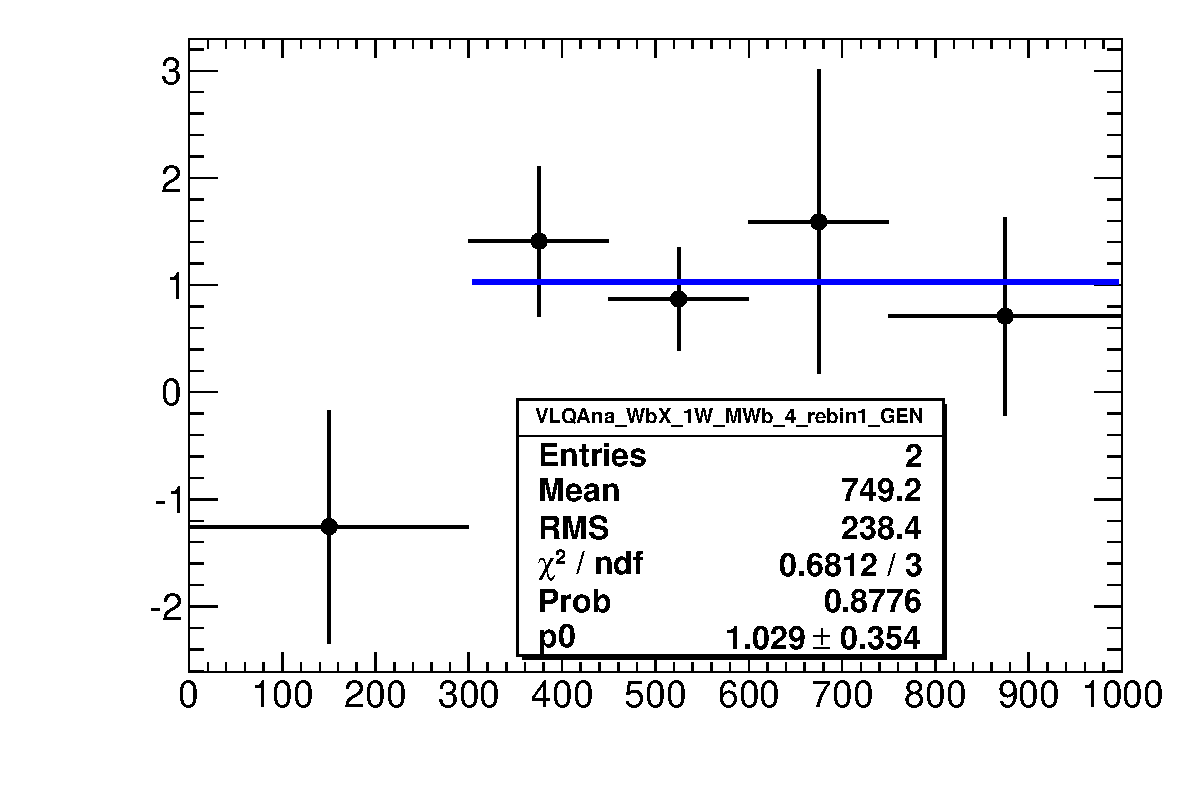
\includegraphics[width=0.33\textwidth]{wbx_analysis_14ifb/figures/ttbarModRatio/GEN_RATIO.eps} &
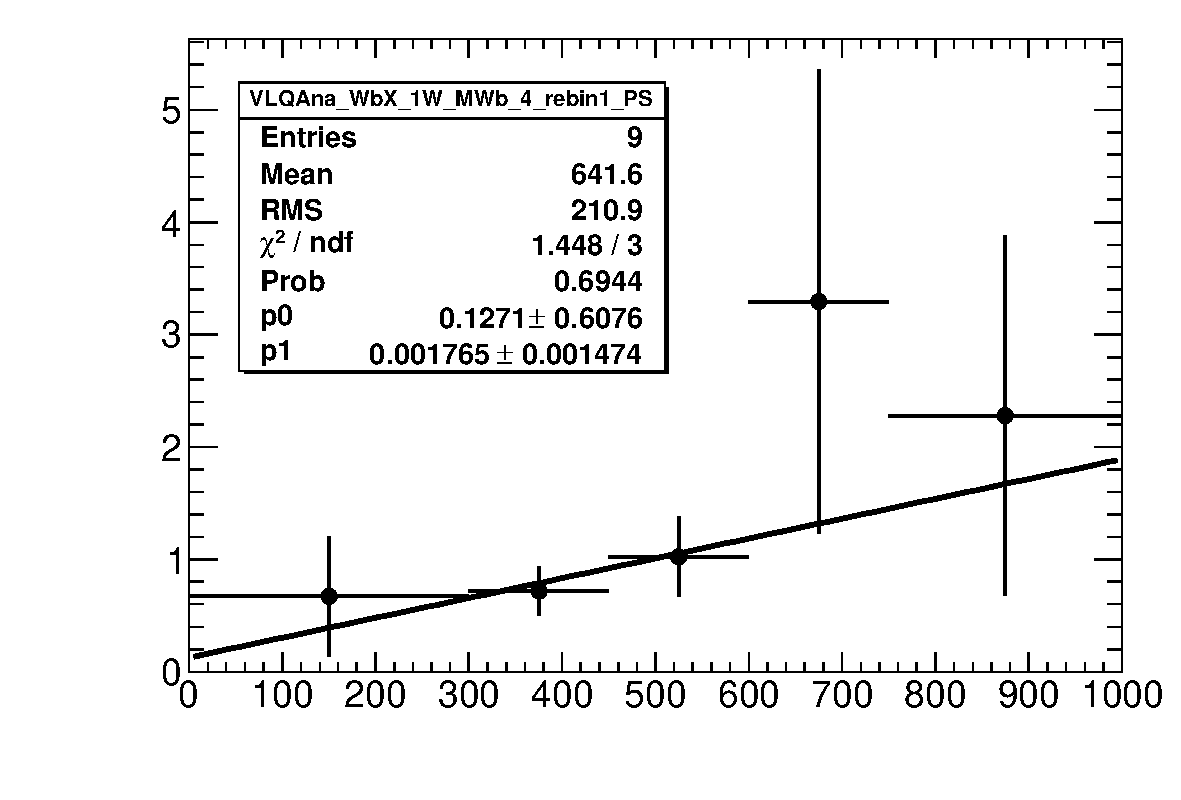
\includegraphics[width=0.33\textwidth]{wbx_analysis_14ifb/figures/ttbarModRatio/PS_RATIO.eps} &
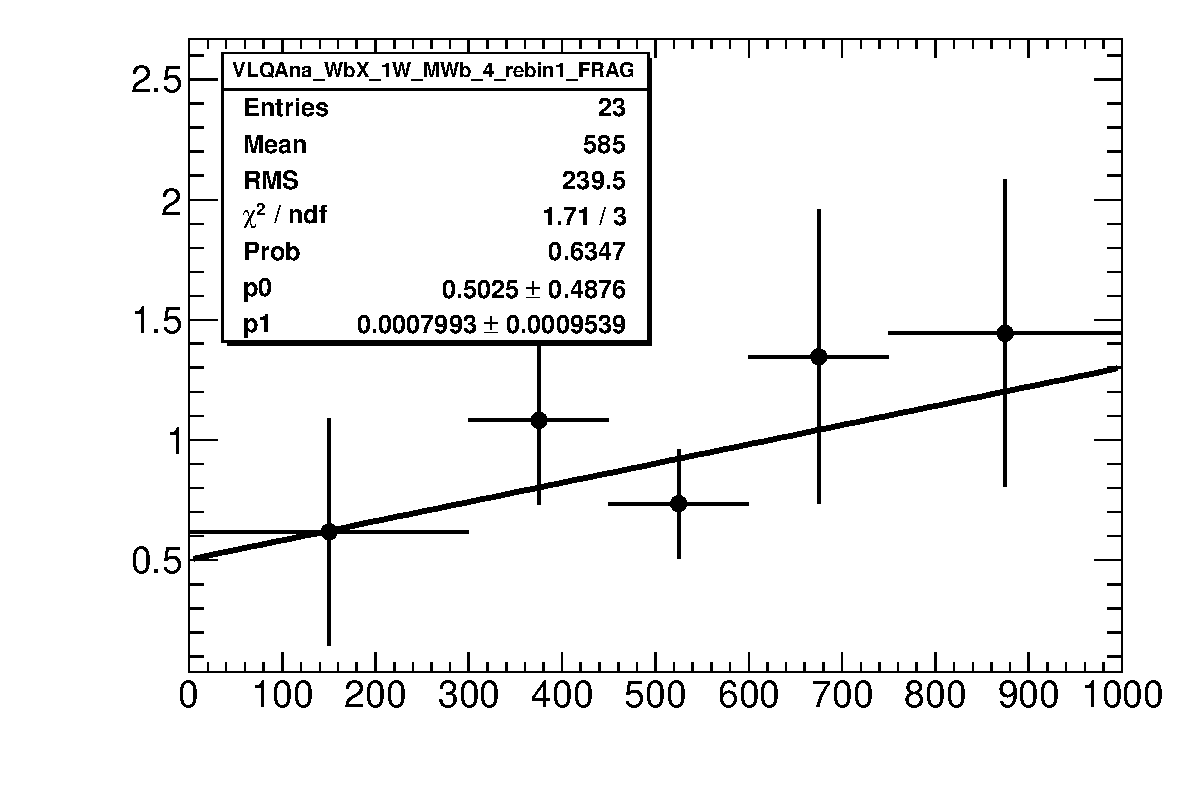
\includegraphics[width=0.33\textwidth]{wbx_analysis_14ifb/figures/ttbarModRatio/FRAG_RATIO.eps} \\
(a) & (b) & (c) \\
\end{tabular}\caption{\small {Ratio of unit-normalized final discriminant between alternative models:
(a) \texttt{mc@nlo} /\texttt{PowHeg+Herwig}  to derive the NLO event generator systematic,
(b) \texttt{AcerMC+lessPS} /\texttt{AcerMC+morePS}  to derive the NLO event generator systematic, and
(c) \texttt{PowHeg+Herwig} /\texttt{PowHeg+Pythia}  to derive the parton shower+fragmentation systematic.
All samples used are AFII.
Also shown are fits to low-order polynomials in order to derive smooth shape systematics.}}
\label{fig:ttbarmodel_ratios}
\end{center}
\end{figure}
%%%%%%%%%%%%%%
\fi

\subsection{$V$+jets Modelling}

The effect of systematic uncertainties affecting the 
modeling of the $V$+jets bacground kinematics by the \texttt{Alpgen}
generator is assessed by changing the factorization scale from the nominal
choice, $Q^2 =m_{\rm W}^2+\sum m_{\rm T}^2$, to $Q^2 =m_{\rm W}^2+p_{\rm T,W}^2$. 
The resulting variation is then symmetrized.
%The variations are implemented via a per-event weight computed as a function of leading jet $\pt$. For more information see Ref.~\cite{WjetsReweighting}.
%{\bf Caveat: currently only the iqopt3 uncertainty is being considered. The ptjmin10 uncertainty will be included in the next iteration.}



\subsection{Overall effect of systematic uncertainties}\label{sec:wbxALLSYS}

In Table~\ref{tab:SystSummary} the final results on
the effect of the different systematic uncertainties affecting
the \wbx\ analysis are reported. It can be seen that the main
contributions come from jet energy scale and resolution,
\btag ging efficiency and, in the case of the \ttbar\ 
background, from the uncertainty on the Monte Carlo modeling
of the simulated \ttbar\ sample.

\begin{table}[htb]
\centering
\resizebox{1.\textwidth}{!}{
\begin{tabular}{l*{3}{c}}
\toprule
 & $\T\bar{\T}$ ($600\gev$) \rule{0pt}{2.6ex} \rule[-1.2ex]{0pt}{0pt} & $t\bar{t}$ & Non-$t\bar{t}$\\
\midrule
\multicolumn{4}{c}{Uncertainties [\%] affecting only the normalisation of the $m_{\rm reco}$ distribution:}\\
Luminosity & +3.6/-3.6 & +3.6/-3.6 & +3.6/-3.6\\
Lepton trigger, reconstruction and ID efficiency & +2.0/-2.0 & +2.0/-2.0 & +2.0/-2.0\\
$t\bar{t}$ cross section & -- & +10/-11 & --\\
\midrule
\multicolumn{4}{c}{Uncertainties [\%] affecting both normalisation and shape of the $m_{\rm reco}$ distribution:}\\
Jet energy scale & +6.6/-8.4 & +15/-15 & +33/-22\\  
Jet energy resolution & +8.4/-8.4 & +3.6/-3.6 & +9.3/-9.3\\ 
Jet identification efficiency & +2.3/-2.7 & +2.3/-2.5 & +1.9/-2.6\\  
$b$-quark tagging efficiency & +6.7/-7.3 & +6.7/-8.9 & +1.8/-2.2\\  
$c$-quark tagging efficiency & +1.6/-1.6 & +4.1/-4.1 & +5.6/-5.6\\  
Light-jet tagging efficiency & +0.3/-0.3 & +0.7/-0.7 & +2.7/-2.7\\  
$t\bar{t}$ modelling: NLO MC generator & -- & +48/-48 & --\\  
$t\bar{t}$ modelling: parton shower and fragmentation & -- & +25/-25 & --\\  
$t\bar{t}$ modelling: initial and final state QCD radiation & -- & +8.8/-8.8 & --\\   
$W$+jets normalisation & -- & -- & +8.9/-7.8\\  
$W$+heavy-flavor fractions & -- & -- & +18/-19\\  
$W$+jets modelling: scale variation & -- & -- & +11/-11\\  
$Z$+jets cross section & -- & -- & +1.1/-1.1\\ 
Single top cross section & -- & -- & +1.9/-1.5\\  
Diboson cross section & -- & -- & $<0.1\%$\\  
$t\bar{t}V$ cross section & -- & -- & +1.5/-1.5\\  
\midrule
Total & +14/-15 & +59/-59 & +42/-35\\
\bottomrule
\end{tabular}}
\caption{List of all systematic uncertainties (in \%) considered in the analysis, indicating which ones are treated
as normalisation and/or shape uncertainties, with their impact on normalisation in the case of the 
\tight\ selection, for signal and backgrounds. The signal given here is a chiral fourth-generation $T$ quark with mass $m_{T}=600\gev$.}
%\caption{List of all systematic uncertainties (in \%) considered in the analysis, indicating which ones are treated
%as normalisation and/or shape uncertainties, with their impact on normalisation in the case of the 
%\tight\ selection, for signal and backgrounds. The signal corresponds to a chiral fourth-generation $\T$ quark with mass $m_{\T}=600\gev$.}
\label{tab:SystSummary}
\end{table}



\section{Results}\label{sec:wbxRES}


In the \wbx\ analysis no significant excess of data over the 
expected background has been observed in the \mreco\ spectra 
of Figure~\ref{fig:mreco}.
Three configurations have been tested to derive the final
results of this search, namely: \loose\ selection using $m_{\rm reco}$ and profiling of overall $t\bar{t}$ yield (``\loose''); \tight\ selection using $m_{\rm reco}$
(``\tight''); \tight\ selection  considering just the overall yield and not 
the shape of $m_{\rm reco}$ (``\tight\ cut-and-count'').
The expected value of $CL_{\rm s}$ (see Section~\ref{sec:cls})
as a function of $m_{\T}$ is
used to choose the best performing strategy.
As was shown in Table~\ref{tab:SystSummary}, the prediction for 
the $t\bar{t}$ background is affected by 
large systematic uncertainties originating from \btag ged jet 
identification efficiency, 
jet energy calibration and resolution and physics modeling in the Monte
Carlo generators. 
In the case of the \loose\ selection configuration the low-mass sideband
region dominated by $t\bar{t}$ can be used to exploit the available data 
statistics to reduce the degrading 
impact of systematic uncertainties on the sensitivity of the search. 
This is accomplished by fitting, during the statistical analysis,
a single nuisance parameter representing a scaling factor on 
the overall $t\bar{t}$ yield. Such procedure is
not possible in the case of the \tight\ selection, where no
sidebands are present as its selection is designed 
to achieve a very high background rejection and high signal-to-background ratio.

As can be seen in Figure~\ref{fig:cls_study}, the \tight\ configuration using 
\mreco\ distribution information achieves an expected
exclusion for a chiral fourth-generation $\T$ quark which is $\sim 50\gev$ 
higher than the reach of both the
\loose\ and \tight\ cut-and-count analyses, whose sensitivies are comparable.
Therefore, the \tight\ selection is chosen 
{\it a priori} to obtain the main result of this search.

\begin{figure}[htb]\begin{center}
	\subfigure{
  	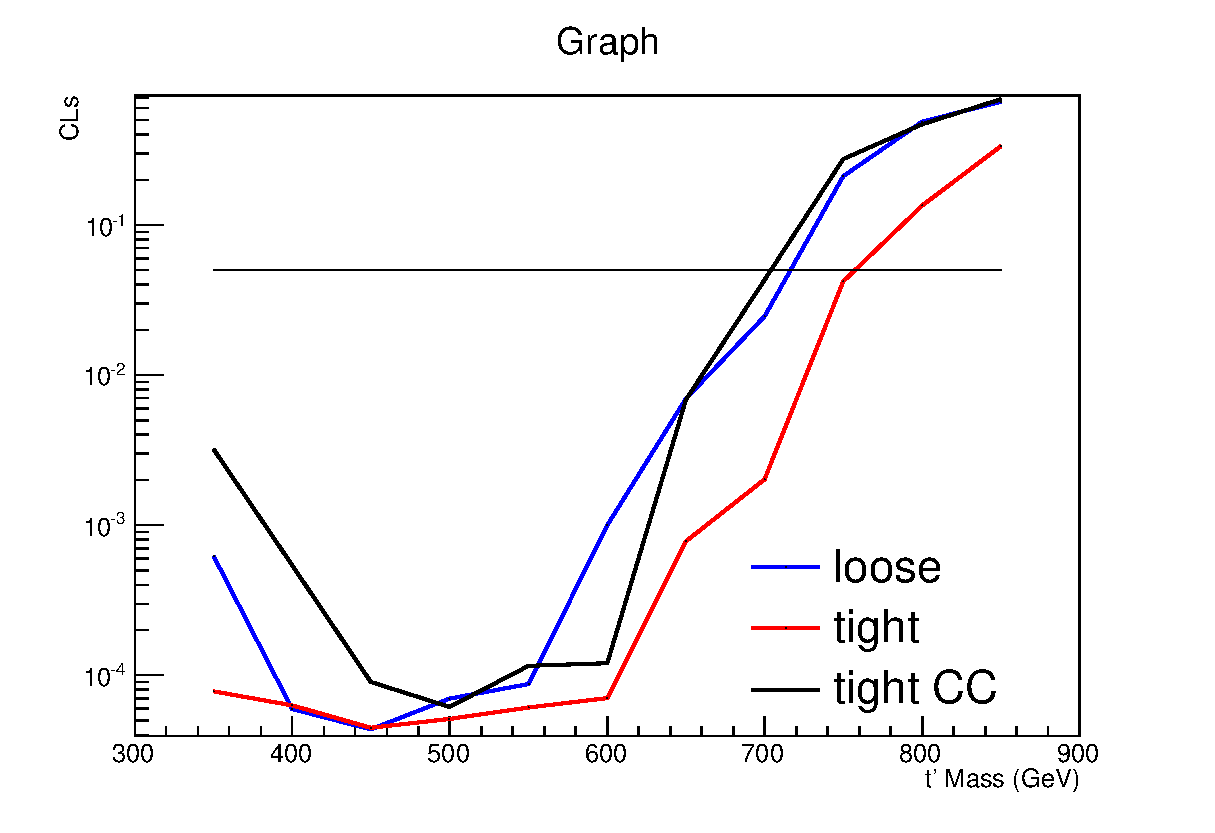
\includegraphics[width=0.7\textwidth]{results/figures/CLs_versus_Mass.eps}}
	\caption{Expected $CL_{\rm s}$ as a function of $m_{\T}$ taking into account systematic uncertainties.
Compared are three possible configurations for the analysis (see text for details).\label{fig:cls_study}}
\end{center}\end{figure}


The observed and expected upper limits on the \TTbar\ production cross section 
times branching fraction as a function of $m_{\T}$ are shown in 
Figure~\ref{fig:limits1D_wbx} for the two chosen benchmark scenarios,
namely the chiral model with 100\% BR($T\to Wb$) and the weak-isospin singlet 
model.
These results include both statistical and systematic uncertainties,
and the consistency of the data with the background prediction is 
assessed following the concepts presented in Section~\ref{sec:cls}
by computing the $p$-value under the background-only hypothesis
(1-$CL_{\rm b}$) for each point of the two-dimensional plane 
(each point corresponding to a signal scenario) and for every heavy 
quark mass point considered (one two-dimensional plane is built for each
$m_T$ value). The smallest $p$-value found is of 0.095 for a vector-like
top-partner with mass $m_{\T}=350\gev$, $BR(\T \to Zt)=0.9$ 
and $BR(\T \to Wb)=BR(\T \to Ht)=0.05$, which corresponds to a 
significance of 1.7 standard deviations above the 
background-only prediction, which is, therefore, not significant.
For a chiral fourth-generation $\T$ quark, an observed (expected) 95\%  CL  limit 
$m_{\T}>740\,(770)\gev$ is obtained for the central value of the 
theoretical cross section.
This result can also be applied to a $Y$ vector-like quark with electric charge of
$-4/3$ and decaying into a $W^-$ boson and a $b$ quark.
For a vector-like singlet $\T$ quark, an observed (expected) 95\%  CL  limit 
$m_{\T}>505\,(630)\gev$ is obtained for the central value of the 
theoretical cross section.

%To assess the impact of the systematic uncertainties on the limit,
%the result has been compared with what is obtained including in the
%analysis only the statistical errors and it was found that systematic
%uncertainties give a degradation of the expected cross section
%limit by $\sim$50\% for the higher $m_{\T}$ values used.
\begin{figure}[h!tb]
\begin{center}
\subfigure[]{\label{fig:limits1D_wbx_chiral}
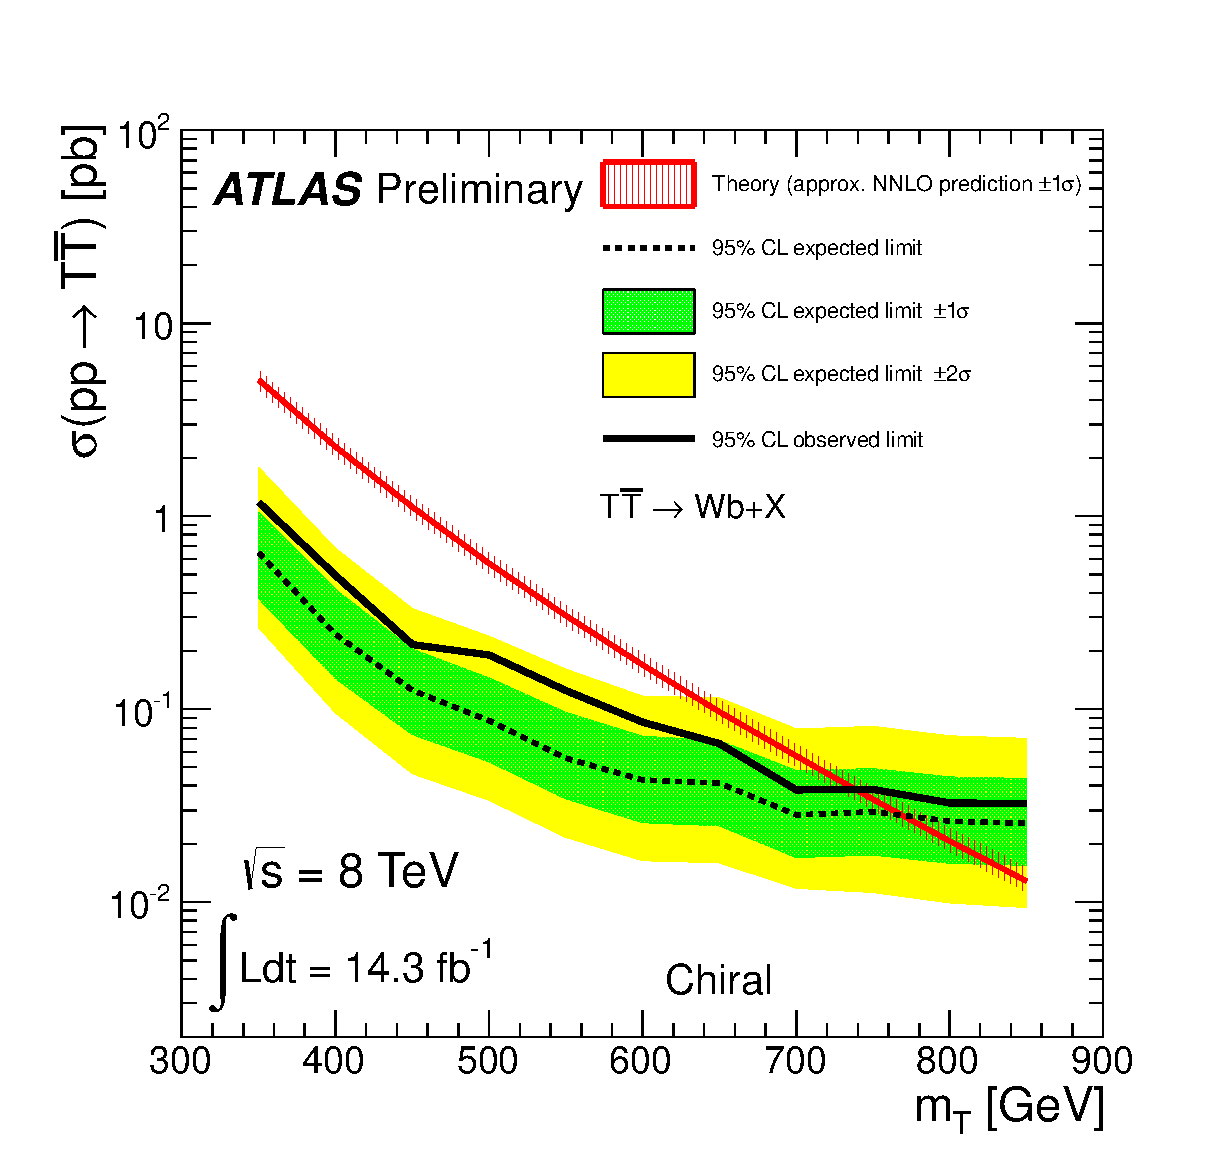
\includegraphics[width=0.45\textwidth]{results/figures/NewttbarMod/lim_chiral_bin1_WbX.eps}}
\subfigure[]{\label{fig:limits1D_wbx_singlet}
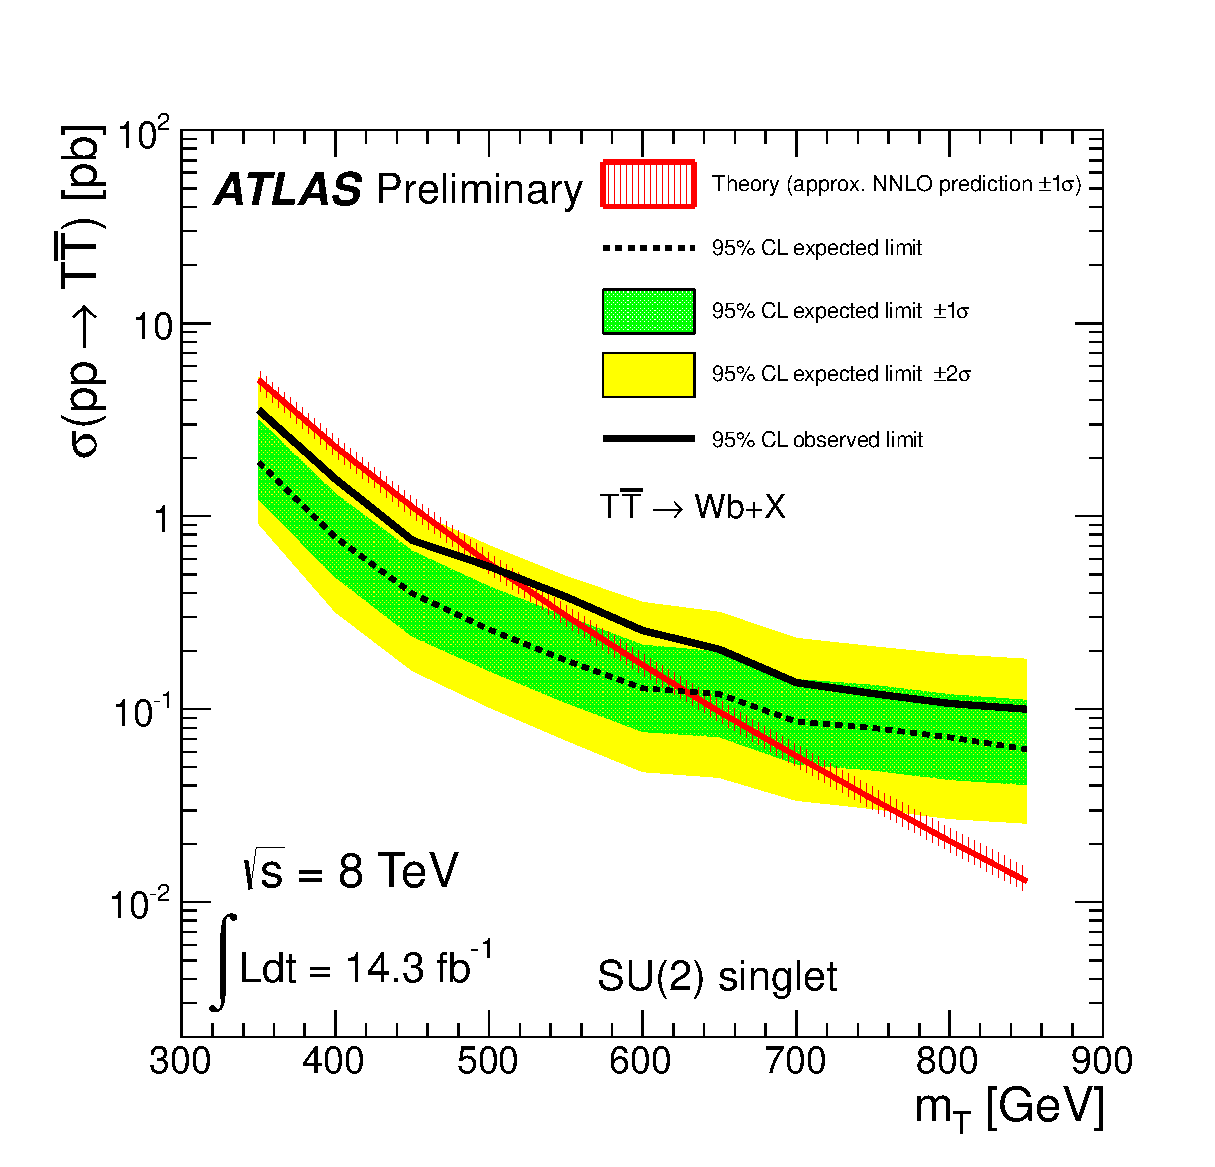
\includegraphics[width=0.45\textwidth]{results/figures/NewttbarMod/lim_singlet_bin1_WbX.eps}}
\caption[bla]{Observed (solid line) and expected (dashed line) 95\% CL upper limits on the $\T \bar{\T}$ cross section times branching fraction
for (a) a chiral fourth-generation $\T$ quark and (b) a vector-like singlet $\T$ quark  as a function of the $\T$ quark mass. 
The surrounding shaded bands correspond to the $\pm1$ and $\pm2$ standard deviations around the expected limit. 
The thin red line and band show the theoretical prediction and its $\pm1$ standard deviation uncertainty.

\label{fig:limits1D_wbx}}
\end{center}
\end{figure}


Concerning the quasi-model independent strategy, 
we recall here that in the two-dimensional plane the gray area
corresponds to the unphysical region where the sum of BRs
exceeds unity. In every plane two benchmark models are indicated
as a plain circle and star symbols, corresponding respectively to the
weak-isospin singlet and doublet scenario BRs values as computed by the
\texttt{PROTOS} event generator.
To probe the full plane the signal samples are reweighted by the ratio
of desired branching ratio to the original branching ratio generated
by \texttt{PROTOS} and the complete analysis are repeated in each point.
The  95\% CL exclusion limits  obtained in the scan of the two-dimensional
plane by varying the mixing of the three decay channel contributions for
different values of $m_{\T}$ are shown in Figure~\ref{fig:limits2D_wbx}. 
This plot reads as follow: taking for instance the $600\gev$ 
vector-like top partner, a heavy quark with
$BR(\T\to W b)>0.7$ is excluded at $\geq 95\%$ CL, 
regardless of the value of the vector-like quark branching ratios to $Ht$ and $Zt$.  
%All the decay modes contribute to the final sensitivity when setting limits.
%For example, assuming $m_{t^\prime}=600\gev$, 
%the acceptance times efficiency of the {\sl tight} selection is 2.45\%, 0.64\%, 0.47\%, 0.10\%, 0.18\% and 0.16\%, for 
%decays to $WbWb$, $WbZt$, $WbHt$, $ZtZt$, $ZtHt$ and $HtHt$, respectively.


\begin{figure}[h!bt]
\begin{center}
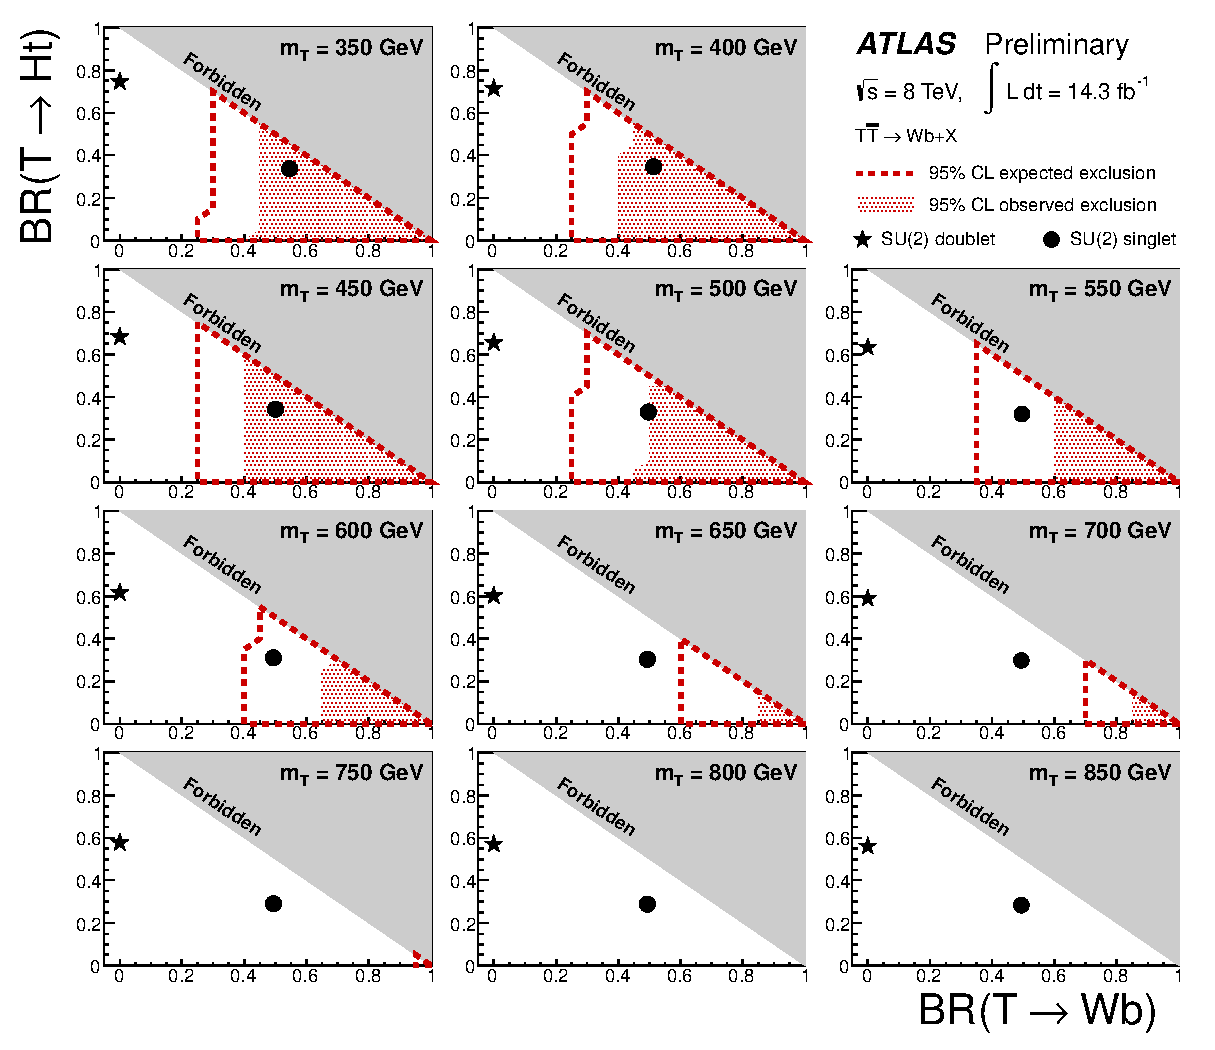
\includegraphics[width=0.9\textwidth]{results/figures/NewttbarMod/lim_Scan2D_tight_Bin1.eps}
\caption{
Observed (red filled area) and expected (red dashed line) 95\% CL exclusion in the plane of
$BR(\T \to Wb)$ versus $BR(\T \to Ht)$, for different values of the vector-like $\T$ quark mass.
\label{fig:limits2D_wbx}}
\end{center}
\end{figure}













